\documentclass[12pt]{report}
\usepackage{graphicx}
\usepackage{hyperref}
\usepackage{setspace}
\usepackage{amsmath}
\usepackage{enumitem}
\usepackage{float}
\usepackage{subcaption}
\usepackage{multirow}
\usepackage{adjustbox}
\usepackage{textcomp}
\usepackage{lipsum}
\usepackage{color}
\usepackage{sectsty}
\usepackage[nottoc]{tocbibind}
\usepackage{grffile}
\usepackage{fancyhdr}
\usepackage{acro}
\usepackage[a4paper,includeheadfoot,margin=2.5cm]{geometry}
\pagestyle{fancy}
\usepackage{titlesec}
\usepackage{graphicx}
\usepackage{xcolor}
\usepackage{dirtree}
\usepackage{amssymb}
\usepackage{tikz}
\usepackage{pgfplots}
\graphicspath{{images/}}
\renewcommand{\headrulewidth}{0pt}
\usepackage{listings}
\usepackage{algorithm}
\usepackage[noend]{algpseudocode}
\usepackage{tabu}
\usepackage[scientific-notation=true]{siunitx}
\usepackage{hyperref}
\usepackage{microtype}
\usepackage{tikzsymbols}
\usepackage{makecell}
\usetikzlibrary{matrix,chains,positioning,decorations,arrows}
\emergencystretch=1em
\newcolumntype{M}[1]{>{\centering\arraybackslash}m{#1}}
\newlist{steps}{enumerate}{1}
\setlist[steps, 1]{label = Step \arabic*:}
\newcommand\myicon[1]{{\color{#1}\rule{2ex}{2ex}}}
\newcommand{\myfolder}[2]{\myicon{#1}\ {#2}}
\restylefloat{table}
%New colors defined below
\definecolor{codegreen}{rgb}{0,0.6,0}
\definecolor{codegray}{rgb}{0.5,0.5,0.5}
\definecolor{codeyellow}{rgb}{0.85, 0.65, 0.13}
\definecolor{backcolour}{rgb}{0.95,0.95,0.92}

%Code listing style named "mystyle"
\lstdefinestyle{mystyle}{
	backgroundcolor=\color{backcolour}, commentstyle=\color{codegreen},
	keywordstyle=\color{blue},
	numberstyle=\tiny\color{codegray},
	stringstyle=\color{codeyellow},
	basicstyle=\footnotesize,
	breakatwhitespace=false,         
	breaklines=true,                 
	captionpos=b,                    
	keepspaces=true,                 
	numbers=left,                    
	numbersep=5pt,                  
	showspaces=false,                
	showstringspaces=false,
	showtabs=false,                  
	tabsize=2
}

%"mystyle" code listing set
\lstset{style=mystyle}

\usepackage[toc,page]{appendix}
%\usepackage[sorting=none]{biblatex}
%\addbibresource{ref.bib}

\DeclareAcronym{ML}{
	short = ML,
	long  = Machine Learning,
	class = abbrev
}
\DeclareAcronym{SL}{
	short = SL,
	long  = Supervised Learning,
	class = abbrev
}
\DeclareAcronym{UL}{
	short = UL,
	long  =Unsupervised Learning,
	class = abbrev
}
\DeclareAcronym{DL}{
	short = DL,
	long  = Deep Learning,
	class = abbrev
}
\DeclareAcronym{CNN}{
	short = CNN,
	long  = Convolutional Neural Network,
	class = abbrev
}
\DeclareAcronym{RNN}{
	short = RNN,
	long  = Recurrent Neural Network,
	class = abbrev
}
\DeclareAcronym{THS}{
	short = THS,
	long  = Twitter Health Surveillance,
	class = abbrev
}
\DeclareAcronym{HDFS}{
	short = HDFS,
	long  = Hadoop Distributed File System,
	class = abbrev
}
\DeclareAcronym{YARN}{
	short = YARN,
	long  = Yet Another Resource Negotiator,
	class = abbrev
}
\DeclareAcronym{NIH}{
	short = NIH,
	long  = National Institutes of Health,
	class = abbrev
}
\DeclareAcronym{AI}{
	short = AI,
	long  = Artificial Intelligence,
	class = abbrev
}
\DeclareAcronym{US}{
	short = US,
	long  = United States,
	class = abbrev
}
\DeclareAcronym{NSF}{
	short = NSF,
	long  = National Science Foundation,
	class = abbrev
}
\DeclareAcronym{CSV}{
	short = CSV,
	long  = Comma Separated Values,
	class = abbrev
}
\DeclareAcronym{API}{
	short = API,
	long  = Application Program Interface,
	class = abbrev
}
\DeclareAcronym{GPU}{
	short = GPU,
	long  = Graphic Processing Unit,
	class = abbrev
}
\DeclareAcronym{NLP}{
	short = NLP,
	long  = Natural Language Processing,
	class = abbrev
}
\DeclareAcronym{MLP}{
	short = MLP,
	long = Multilayer Perceptron,
	class = abbrev
}
\DeclareAcronym{UPRM}{
	short = UPRM,
	long  = University of Puerto Rico Mayag\"uez Campus,
	class = abbrev
}
\DeclareAcronym{LSTM}{
	short = LSTM,
	long  = Long Short-Term Memory,
	class = abbrev
}
\DeclareAcronym{GRU}{
	short = GRU,
	long  = Gated Recurrent Unit,
	class = abbrev
}
\DeclareAcronym{NLTK}{
	short = NLTK,
	long  = Natural Language Toolkit,
	class = abbrev
}
\DeclareAcronym{CUDA}{
	short = CUDA,
	long  = Compute Unified Device Architecture,
	class = abbrev
}
\DeclareAcronym{SQL}{
	short = SQL,
	long  = Structured Query Language,
	class = abbrev
}
\DeclareAcronym{CPU}{
	short = CPU,
	long  = Central Processing Unit,
	class = abbrev
}
\DeclareAcronym{OS}{
	short = OS,
	long  = Operating System,
	class = abbrev
}
\DeclareAcronym{JSON}{
	short = JSON,
	long  = JavaScript Object Notation,
	class = abbrev
}
\DeclareAcronym{ReLU}{
	short = ReLU,
	long = Rectified Linear Unit,
	class = abbrev
}

\pgfplotsset{compat=1.14}
\setlength{\headheight}{15pt}
\setcounter{secnumdepth}{3}
\begin{document}
	\newtheorem{definition}{Example}
	
	\newtheorem{property}{Property}
	
	\pagenumbering{roman}%
	
	\begin{titlepage}
		\centering 
		{\LARGE \textbf {Finding Similar Tweets Within Health Related Topics}\par}
		\vspace{1cm}
		{By\par}
		{Danny Gilberto Villanueva Vega\par}    
		{A thesis submitted in partial fulfillment of the requirements for the degree \par}
		\vspace{.1cm}
		{of\par}
		\vspace{.1cm}
		{MASTER OF SCIENCE\par}
		{in\par}
		{COMPUTER ENGINEERING\par}
		{UNIVERSITY OF PUERTO RICO
			\\MAYAG\"UEZ}{  CAMPUS\par}
		{2019}
		\vspace{.1cm}
		\begin{flushleft}
			Approved by:\\
			\vspace{1cm}
		\end{flushleft}
		\begin{tabular}{l c c c c c r}
			
			\rule{2.5in}{.1pt} & & & &  &\rule{2in}{.1pt}\\
			Manuel Rodr\'iguez Mart\'inez, Ph.D. & & & &  &Date\\
			President, Graduate Committee\\
			\vspace{.3cm}\\
			\rule{2.5in}{.1pt}& & & &  &\rule{2in}{.1pt}\\
			Wilson Rivera Gallego, Ph.D. & & & &  &Date\\
			Member, Graduate Committee\\
			\vspace{.3cm}\\
			\rule{2.5in}{.1pt} & & & &  &\rule{2in}{.1pt}\\
			Pedro I. Rivera Vega, Ph.D. & & & &  &Date\\
			Member, Graduate Committee\\
			\vspace{.45cm}\\
			\rule{2.5in}{.1pt} & & & &  &\rule{2in}{.1pt}\\
			Ivette Cruzado, Ph.D. & & & &  &Date\\
			Graduate School Representative\\
			\vspace{.45cm}\\
			\rule{2.5in}{.1pt} & & & &  &\rule{2in}{.1pt}\\
			Bienvenido J Velez Rivera, Ph.D. & & & &  &Date\\
			Dean of Engineering \\
		\end{tabular}
	\end{titlepage}
	
	\setcounter{page}{2}
	
	\addcontentsline{toc}{chapter}{Abstract}
	\begin{center}
		\doublespacing
		Abstract of Thesis Presented to the Graduate School\\
		of the University of Puerto Rico in Partial Fulfillment of the\\
		Requirements for the Degree of Master of Science in Computer Engineering\\
		\vspace{.1cm}
		\large\textbf {Find Similar Tweets Within Health Related Topics}
	\end{center}
	\doublespacing
Social networks have become a very important means to facilitate the creation and sharing of information, ideas, news, and opinions on many topics.  They also provide real-time information on sales, marketing, politics, natural disasters, and crisis situations, among others. These networks include Facebook, Twitter, WhatsApp, and Instagram, to name a few. In this work, we shall focus our efforts on the Twitter social network. This network provides a mechanism for people to express their views using short messages (i.e., 280 characters)
	called {\em tweets}. In this project, we investigate and implement text similarity neural network models in such a way that we can: 1) know if they are related or not with a disease, 2) group similar tweets to those that we have already captured, analyzed or stored, and 3) find similarity index between tweets using different learning algorithms. We based our work on, semantic similarity approaches and text similarity measures using Deep Learning algorithms to deliver reliable information about health-related topics.

	\par
	\clearpage
	
	\addcontentsline{toc}{chapter}{Abstract (Spanish)}
	\begin{center}
		Resumen de tesis presentada a la Escuela Graduada\\
		de la Universidad de Puerto Rico como requisito parcial de los\\
		requerimientos para el grado de Maestr\'ia en Ciencias en Ingenier\'ia de Computadoras\\
		
		\vspace{.1cm}
		\large\textbf {Encontrar tweets similares en temas relacionados con la salud}
	\end{center}
	\doublespacing
Las redes sociales se han convertido en un medio muy importante para crear y compartir informaci\'on, ideas, noticias y opiniones sobre muchos temas. Estas tambi\'en proporcionan informaci\'on en tiempo real sobre ventas, mercadotecnia, pol\'itica, desastres naturales y situaciones de crisis, entre otros. Estas redes incluyen Facebook, Twitter, WhatsApp e Instagram, por nombrar algunas. En este trabajo, centraremos nuestros esfuerzos en la red social Twitter. Esta red proporciona un mecanismo para que las personas expresen sus puntos de vista mediante mensajes cortos (no m\'as de 280 caracteres)
llamados {\em tweets}. En este proyecto, investigamos e implementamos modelos de redes neuronales de similitud de texto de manera que podamos: 1) saber si est\'an relacionados o no con una enfermedad, 2) agrupar tweets similares a los que ya hemos capturado, analizado o almacenado y 3) encontrar el \'indice de similitud entre los tweets que utilizan diferentes algoritmos de aprendizaje. Basamos nuestro trabajo en los enfoques de similitud sem\'antica y las medidas de similitud de texto utilizando algoritmos de ``Deep Learning" para proporcionar informaci\'on confiable sobre temas relacionados a la salud.

	\par
	\clearpage
	
	\vspace*{\fill}
	\begin{table}[H]
		\centering
		\begin{adjustbox}{max width=\textwidth }
			\begin{tabular}{c}
				Copyright \textcopyright\hspace{0.15cm}2019 \\
				\textit{by}\\
				\textit{Danny Gilberto Villanueva Vega}\\
			\end{tabular}
		\end{adjustbox} 
	\end{table}
	\vfill
	\clearpage
	
	\vspace*{\fill}
	\begin{center}
		\textit{DEDICATION}\\
		\vspace{2cm}
		\textit{To my Mom, Carin Vega P\'erez. To my sister, Emyli S Rodriguez Vega.}
	\end{center}
	\vfill
	\clearpage
	
	\vspace*{\fill}
	\addcontentsline{toc}{chapter}{Acknowledgment}
	
	\begin{center}
		\Large \textbf{Acknowledgments}
	\end{center}
	First of all thank God for giving me health, strength and the desire to persevere forever. I also want to thank my mother Carin and my sister Emily for the love, affection and unconditional support they have always given me, without which it would have been more difficult to achieve this goal.
	
	I would like to express my sincere gratitude to my adviser Manuel Rodriguez, for the opportunity to work with him, for his patience, motivation, teaching during the whole process of the research and his support during my master's studies. His guidance and advice was very helpful in all aspects of the research and thesis presentation.
	
	I would also like to thank the 54 labelers, which were students from \ac{UPRM} that were enrolled in the course ``Introduction to Database Systems''
	
	This research is supported by the \ac{US} National Library of Medicine of the \ac{NIH} under award number R15LM012275. The content is solely the responsibility of the authors and does not necessarily represent the official views of the \ac{NIH}. Some results presented in this thesis were obtained using the Chameleon Cloud supported by the \ac{NSF}.
	\vfill
	\doublespacing
	
	\tableofcontents{}
	
	\newpage
	\printacronyms[include-classes=abbrev,name=List of Abbreviations]
	\newpage
	\listoffigures{}
	\newpage
	\listoftables{}
	
	\newpage
	\titlespacing{\chapter}{0pt}{*1}{*1}
	
	\fancyhf{}
	\fancyhead[R]{\thepage} 
	\renewcommand{\figurename}{Fig}
	\pagenumbering{arabic}
	\onehalfspacing
	\chapter{Introduction}\label{Chapter 1}
	\doublespacing
	
	\section{Motivation}
	Social networks have become a very important means to facilitate the creation and sharing of information, ideas, news, and opinions on many topics.  They also provide real-time information on sales, marketing, politics, natural disasters, and crisis situations, among others. These networks include Facebook, Twitter, WhatsApp, and Instagram, to name a few. 
	
	In this work, we shall focus our efforts on the Twitter social network. This network provides a mechanism for people to express their views using short messages (i.e., 280 characters)
	called {\em tweets}. 
	Users of this network can find each other messages without the need of becoming ``friends'', as it happens in other networks. The analysis of these tweets can enable us to understand the current situation regarding certain topics, for example, discussions related to medical topics (e.g., ``flu'').
	Users can monitor and find patterns that give information about some type of disease being discussed in the social network. In addition, it is possible to detect the sentiment, ``mood'' of the people discussing a specific topic.

	In the health care domain, searching text in social medias, blogs and newspapers can provide clues about the diseases that are being talked about 
	by citizens of a region. For example, an increase in messaging related with a disease (e.g., Measles) could indicate that people are concerned 
	due to some outbreak and are looking for more information about symptoms and treatments. 
		
	For the analysis of all this available information it is {\em necessary to group or categorize the text along similarities in structure and/or meaning}. However, this is a challenging task, due to the complexity/ambiguity introduced by  spelling errors or the use of informal language (``slang'').  In the case of tweets, the small size of the message often makes it difficult to analyze without the context provided by previous messages or user interactions. Making use of the data stored in the  \ac{THS} System from the \ac{UPRM}, as one of our sources, it is possible to process all the information easily and quickly, and use it to analyze and process the data using  \ac{ML} algorithms, a popular branch of \ac{AI} systems. In particular, deep neural network models can be trained to learn to detect whether tweets are related to  medical conditions. In addition, these models can be trained to  find semantic similarity in a collection of tweets.
	
	
	%The view of the world has changed with the recent progress and ubiquity   of \ac{AI} systems in our lives. We can say that we now live in a new world surrounded by \ac{ML} (e.g. Amazon Alexa, writing correctors). Companies like Google, Amazon, Netflix and others are using \ac{AI} algorithms to obtain value and insight of large amount of data that  otherwise would be  impossible to analyze. In particular, search and mining of text data from social media, blogs, and and other sources provided valuable insight to companies about the opinions of customers. 
	%	 The value of the information has been ever the key for the growth of companies; therefore, text analysis is a rough task aim to extract value %information to use in business decisions, however this is challenging job due to complexity of \ac{NLP} a field of \ac{ML}  focuses on analyzing the %human language.
	

	
	%The detection of similarity in texts in their meaning of semantics content is a topic present in many researches because the need to obtain valuable and reliable information from the amount of available data over internet like, communication services (e.g. “Twitter”), feedback user, system log files, customer reviews to mention a few; and the data present in the same company about employees, clients and others. 
	
	In this project, we investigate and implement text similarity neural network models in such a way that we can: 1) know if they are related or not with a disease, 2) group similar tweets to those that we have already captured, analyzed or stored, and 3) find similarity index between tweets using different learning algorithms. We based our work on, semantic similarity approaches and text similarity measures using \ac{DL} algorithms to deliver reliable information to the end user about health-related topics.
	
	
	\section{Objectives}
	
	Our work is rooted in our \ac{THS} project at UPRM, whose goal is to monitor tweets related with medical conditions, and detect instances where
a disease is actively being discussed in a given region.
The main problem that we want to tackle in this project is the development of  \ac{DL} models that can evaluate the similarity between
tweets. Specifically, given an example tweet $T_p$ (``premise tweet"), and  a collection of tweets $T_1, T_2, ..., T_n$, we want to rank the collection of tweets
from the most similar to the least one to $T_p$. In order to do, so {\bf we need to develop a method to measure the similarity between pairs of 
	tweets}. Our goal is to use \ac{DL} to achieve this. 
By using a \ac{DL} model trained to rank tweets based on similarity, users could: 
\begin{itemize}
	\item pick a tweet - the example tweet- that they consider useful for detecting conversations about a given disease and
	\item setup a process to watch the Twitter stream and collect tweets similar  to the example one and visualize these tweets  sorted by 
	relevance of their similarity. The model can be used to compute a similarity score between the example tweets and each tweet read from the stream. Then, sorting can be used to provide a ranked list based on the similarity.
\end{itemize} 

To accomplish this it was necessary investigate the state-of-the-art methods and techniques related to text analysis, and build a robust architecture using \ac{DL} algorithms like, \ac{CNN} and \ac{RNN} on \ac{NLP} approaches,  focusing on text similarity measures.

%As we described in section \ref{sem_sim},   text similarity measures are very difficult to calculate  because it is hard to find the meaning and context match of the two pieces of text. To manage those issues, we use relevant information to find context similarity and syntactical similarity, like the type of disease mentioned in each tweet,  or if the tweet is related to a disease or not. This contextual information can be used as pre-processing step before feeding 
%the tweets to the \ac{DL} model.
%
%
%	REVISE in light of new work
%	\begin{itemize}[nolistsep]
%		\item \textbf{Collect and filter the data file: } We select necessary tweets and filter all them which are related to health disease thereby, we use a clean data as input to train the algorithms to be implemented. Tweets were collected using \ac{THS} System at \ac{UPRM}. In this way, it is convenient to describe the steps through the process of data selection until deliver of final cleaned up inputs. Part of inputs is labeled data by hand; thus, it is necessary a group of people to classify a measure of similarity between tweets that will be used in training sample.
%		\item \textbf{Investigate and implements \ac{DL} algorithms for text similarity measures} It is necessary investigate the state-of-the-art methods and techniques related to text analysis, and then build a robust architecture using \ac{DL} algorithms like, \ac{CNN} and \ac{RNN} on \ac{NLP} approaches,  focusing in text similarity measures. The output of our trained models will be one of two of next options a) there is an acceptable similarity measure between the pair of tweets and, b) no exist enough similarity between the pair of tweets.
%		\item \textbf{Test algorithms in a Big Data environment: } The algorithms will be tested to measure the performance and accuracy of results in \ac{THS} cluster located in the Electrical and Computer Department at \ac{UPRM}. Because \ac{DL} algorithms consume a lot of resources, we also use virtual environments as Chameleon Cloud Platforms to test algorithms with better Graphic Processing Unit (GPU) resources than physical machines.
%	\end{itemize}
	
	\section{Contributions}
	\begin{itemize}[nolistsep]
		
		
		
		\item \textbf{Use-case on social networks application to get valuable information about health topics:}  Data available on the Internet through social networks, entertainment apps and others, can be used in health-related research. In our case,  Twitter is a source of vast amounts of data on different topics that can be transformed into insights about  medical issues. We illustrate  how we can use tweet data about medical conditions to build models that are able to compute the similarity in tweets.These collection of similar tweets  it could be used in the future to support medical applications that try to find trending patterns, 
		anomaly detection, or hidden, repetitive events. 
		%\item \textbf{Present \ac{DL} models for text similarity analysis:} \ac{DL} models are very powerful for analysis of data like images, sound, and text. In this project, we try to use these excellent tools of \ac{ML} to figure out a better text similarity model.
		\item \textbf{Employ Supervised Learning in text similarity tasks:} Most studies about sentence representation (``encoding models'') and text similarity are based on unsupervised learning (usually clustering) because there is not enough labeled data about a specific task to train a model. This happens in our target problem where we want to find similar tweets related with medical conditions. We show the trained models with labeled data in sentence similarity have good performance to be widely adopted for tweet similarity and in others \ac{NLP} tasks.
		%\item \textbf{Use different measure of similarity:} In this project we used three methods to calculate similarity text. Most known is cosine similarity, also Frobenius Distance and our own distance measure called Triangular UL Distance based in part of linear algebra, in a special kind of square matrix called triangular matrix.
		\item \textbf{Present a novel strategy to build similarity models: } We build models with deep \ac{CNN} and \ac{RNN} to obtain acceptable results close to 90\% of accuracy. 
		In order to obtain a model $M$ that can compute the similarity rank between two tweets, we borrow from the strategy in \cite{Wang2014}, and first train a larger model $M'$
that is capable of classifying relative similarity in triplets of tweets. This is a common strategy in \ac{DL}: {\em train a bigger model that does a task in which the model you really want is  
	a sub-task (sub-model)}. This is done because the bigger model might be easier to train on its intended task, or because there is data already available to train the bigger model.  Once the bigger model is trained, the sub-model is taken out and used in standalone fashion. In our specific case, the task that performs model $M$, computing the similarity between two tweets, becomes a sub-task in a bigger
model $M'$ that classifies which of two tweets is more similar to a premise tweet.
		\item \textbf{Present a performance study on the DL similarity models}: We have created a data sets consisting of 11,425 examples, and we use that data set to train our models. Our results show that we can achieve 90\% accuracy on the task of classifying which of two tweets is more similar to a premise tweet.
		For this task, we need to train a sub-model that computes the similarity rank between two tweets as  a value in the range [0,4]. 
		This is a regression tasks and our model have a 0.34 units of Mean Squared Error on a decreasing loss.
	\end{itemize}
	
	\section{Outline}
	The outline of this thesis is as follows. Chapter 2 contains the literature review on concepts of \ac{ML} and \ac{DL} to contextualize our work. In this chapter we also describe topics of \ac{NLP} and text similarity methods. The problem description and the methodology followed to build the similarity models are described in Chapter 3. In Chapter 4, we explain the \ac{ML} architecture, implementation, and  the different \ac{DL} models built using \ac{CNN} and \ac{RNN}. Chapter 5 shows the results on performance and accuracy of all models built in this work. Finally, Chapter 6 shows the conclusions and future work.
	
	\onehalfspacing
	
	\chapter{Literature Review} \label{chapter 2}
	\section{Introduction}
	%Advance of technology has been many changes in the world and our life is now surrounding for \ac{ML} algorithms hence, companies of all sizes are %following the large business' success using \ac{AI} to draw insight that can be used to take better decisions.
	
	The field of \ac{AI} seeks to understand how humans think (``intelligence''), and how to use that knowledge to build programs that show intelligence. 
	Today \ac{AI} is a very wide field, making it difficult to give a simple answer to what its an AI application. However we can mention a few applications that exist today:  autonomous robotic vehicles, speech recognition, autonomous planning and scheduling, game playing, spam fighting, logistics planning, robotics in 
	automation, and machine translation. These applications combine efforts in computer science, engineering, mathematics, and cognitive sciences \cite{Russell2010}.These applications need to process a lot of data, hence it is necessary to automate the process of data acquisition and analysis. 
	Big data analytics is used to for the purpose of data management in this context.  Machine Learning (\ac{ML})  (a subfield of \ac{AI}) provides the tools  that automate the process of learning  how to extract patterns from the raw data to get insights \cite{Kelleher2015}.
	
	Artificial Neural Networks and \ac{DL} are very popular methods in \ac{ML}. Neural Networks are simply a collection of connected computational 
	units that represent abstractly the human brain (“neurons”) and  aim to achieve learning on a specific task \cite{Russell2010}. These neurons are organized and interconnected into layers. Deep learning is the development of complex neural networks that contain many layers of neurons. These networks are computationally expensive to train and require relatively high amounts of training data. But, they can rival human expertise at various taks, such as image classification and language translation.  
	
	In this project we are working on similarity tasks related with text messages from Twitter. This problem bear similarity with many applications of similarity for handwritten digits recognition, image similarity detection from text, and image content search  in  web searchers (e.g. Google, Bing).  Neural Network techniques can be successfully applied for these problems, but to achieve better results and scale to large applications we need used techniques specialized on certain domains, for example in case of \ac{NLP} (``text analysis'') we need methods to process sequential data, like {RNN}, that is a{DL} technique part of {ML} field \cite{Goodfellow2016}.  In the rest of this chapter, we go over background information related with machine learning that is necessary to understand the context and the contributions of our work.
	
	\section{Machine Learning}
	
	Machine learning, \ac{ML}, also known as automated learning, is associated with the concept of making computers learn some tasks without actually 
	programming the computer to do so. Typically, \ac{ML} involves a training phase, where an algorithm is implemented in software and then presented
	with many examples of the task to be learned. The training phase produces a {\em model} which is the trained, ``intelligent" software module that automates some tasks. This model is then
	validated in the second phase, where unseen examples are given to the model and we evaluate its performance. 
	Typically models are evaluated based on either accuracy of prediction (i.e., classification tasks)  or on the mean square error incurred when approximating some quantity (i.e., regression tasks). If multiple, competing  models are trained and validated, then the final selection is done in a third phase called the 
	{\em test phase}, where additional examples are given to the competing models to pick the best one amongst them. 
	Notice that this learning is composed of  input data that represent previous experience, and the model will learn to produce an output based on such input.  \cite{Shai2014}. 
	This learning process is focused on gaining knowledge, understanding, experience, and skills \cite{Nilsson1998} in such a manner its performance improves significantly over time.
	
	%Today we look that \ac{ML} is in many practical applications that we use in frequently in our daily life like: movie recommendation, text translation, speech recognition \cite{Goodfellow2016}, robotic vehicles, autonomous planning and scheduling, diagnosing diseases \cite{Russell2010}. In essence, we are speaking about \ac{ML} when an artificial intelligence system has the ability or capability to get knowledge or find patterns from raw data \cite{Goodfellow2016}. \ac{ML} study data to detect patterns to be able to categorize, predict, identify unknown pattern and detect anomalies or unknown patterns, because Big Data we now have the advantage to process an amount of data, and using {ML} algorithms we can identify new opportunities to solve complex problems like self-driving cars, fraud detection, virtual assistants, resource optimization and more applications \cite{Nevala2017}.
	
	\ac{ML} is a very wide field, for this reason it has branched into several sub-fields related to distinct tasks \cite{Shai2014} and approaches to solve problems. For the study and application of these algorithms,  there are many ways to organize the learning paradigms. The best known are supervised learning and unsupervised learning. This distinction is by what kind of experience they are allowed to have during the training process \cite{Goodfellow2016}. Others kinds of {ML} are semi-supervised learning and reinforcement learning.
	
	
	\subsection{Supervised Learning}
	In Supervised Learning, a model is presented  with pairs of input and output items. Often, the input data items in the pairs are called {\em features}.
	Likewise, the output data items in the pairs are often called  {\em labels}. 
	%Supervised Learning is based in an set of input-output pairs, 
	During training, the model automatically learns   the relationship between the input features and the labels. In essence, the model is learning a  function that maps from the input data to the output data \cite{Russell2010,Kelleher2015}. This kind of learning is only possible if we know the output data \cite{Nilsson1998} and if we have enough examples to train the {ML} algorithm. A good rule of thumb by Professor Andrew Ng, from Stanford University, is to have at least 10,000 examples to train your models. \cite{Stanford2019}
	
	
	\begin{figure}[H]	
		\centering	
		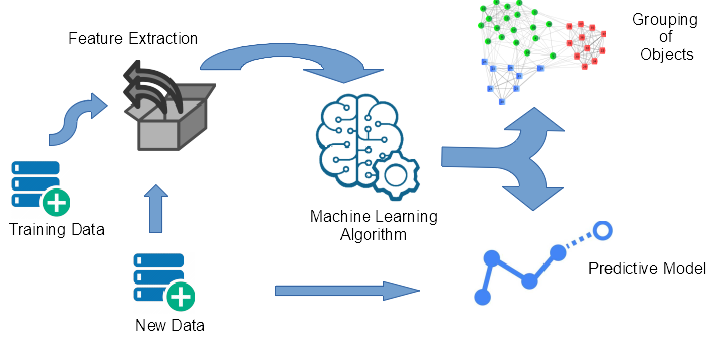
\includegraphics[width=150mm, scale = 1]{images/1_Supervised.png}
		\caption{Supervised Learning Workflow.}
		\label{figure:Supervised_Learning}
	\end{figure}
	
	Figure \ref{figure:Supervised_Learning} shows the process of a supervised learning model. The input of the model is data that contains each element with its respective label. Next the model extracts the most relevant features of the data, to find the relation between input and output, and construct a logical pattern. Finally, the model is trained to learn patterns, generalize data and predict new outputs from  new, unseen, unlabeled data items.
	
	The nature of the labels is dependent upon the type of learning problem being tackled.
	If the supervised tasks involves classification, then the label represents 
	the class or grouping to which the input in the pair belongs. An example classification task will be determining if an image represents a cat or a dog based on the pixels in the image. If the tasks involves regression, then the label represents a quantity associated with the input features. For example, we 
	could predict expected battery life of a lithium battery  as a function of daily depth of discharge.  
	
	%More abstractly, Supervised Learning describe a scenery where the training examples is a set of data that contains the necessary information to identify and associate it to the output value. This information is not available in the test data to which the learned model is being applied. The aim is that the acquired expertise will can predict the expected output \cite{Shai2014}.
	
	%It is called ``supervised'' because the environment provides an extra information, commonly known as labels, the model is trained with input data and target data \cite{Shai2014}. The target value (``label'') is provided by a supervisor who teach to the system what to do \cite{Goodfellow2016} , providing the correct output (``desired output'') as a feedback for reduce error.
	
	%Supervised learning identify correlation and a logical pattern in data from the from state A to state B, after these pattern are learnt, we can transfer learning to solve similar problems \cite{Nevala2017} \cite{Cer2018}. 
	
	Common techniques used for supervised learning are logistic regression, decision trees, neural networks, and support vector machines.
	Supervised learning is used in applications such as risk assessment, digital assitants, speech recognition, language translation, 
	image processing, fraud detection, and  customer segmentation \cite{Nevala2017}.
	
	\subsection{Unsupervised Learning}
	In unsupervised learning, there are no labels in the data. Instead, the model tries to uncover the underlying structure in the data by 
	finding correlations and identifying patterns parsing the available data \cite{Nevala2017}. Unsupervised learning is often used as 
	an initial phase during data analysis to figure out the structure of the data. 
	%
	%%Today Big Data is a great tool that makes possible analyze a great amount of information, faster and easier.  Raw data in many cases is difficult to analyze and many cases we do not have an answer key for our trainable data. In this cases we can use unsupervised learning like an alternative, therefore we can determine 
	%
	%This kind of algorithms learns patterns without an explicit feedback (``label'') \cite{Russell2010}, we only have a training data without target values for them \cite{Nilsson1998}. 
	There is no separation of training data and test data \cite{Shai2014}; all the data is the input for the algorithm. This method is similar to human behavior: when we observe the world, usually we do inferences and group things based on our interaction with the environment.
	This type of learning is refined by exposing the model to  a lot of observations \cite{Nevala2017}.
	
	The most common technique for this learning modality is called {\em clustering}, \cite{Russell2010}, which separates the data into meaningful categories called {\em clusters}. Each cluster is made up of data items that have similar characteristics \cite{Goodfellow2016,Nilsson1998}. This similarity is measured by using a function that computes a similarity metric, often a variation of a distance function. In practice, the items are represented as vectors $v_1,  v_2, ..., v_k$ and the metrics measures how close are to each other in their vector space. Other unsupervised techniques are nearest neighbor mapping, singular value decomposition,  self-organizing maps, Hidden Markov Models, and anomaly detection, to name a few. Their applications are related to market basket analysis, anomaly/intrusion detection, text classification, identifying similarities amongst data elements, sentiment analysis, and so on \cite{Nevala2017,Halibas2018}.
	
	In Figure \ref{figure:Unsupervised_Learning} we show a workflow for unsupervised learning. In this case, we show clustering of documents based on content. First, the text and other features in documents are converted into a vector representation (i.e., one-hot vectors). Next the model extracts the most relevant features of the data,  then a clustering algorithm (e.g., k-means clustering) is used to assign each vector to a cluster. The number of cluster is pre-defined at the start of the learning process.
	Once trained, the model is able to take new data items and cluster them.
	
	\begin{figure}[H]	
		\centering
		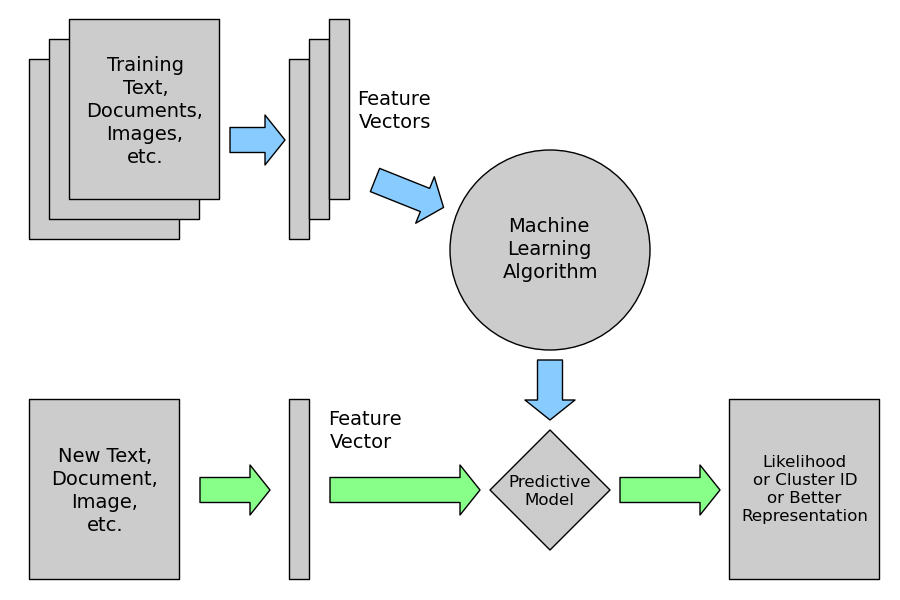
\includegraphics[width=150mm, scale = 1]{images/2-Unsupervised_Learning.png}	
		\caption{Unsupervised Learning Workflow.}	
		\label{figure:Unsupervised_Learning}
	\end{figure}
	
	
	
	\section{Neural Networks}
	An artificial neural network is a very simplified abstract model of a biological brain, an interconnection of processing units with capability to learn patterns, generalize and associate data. A significant aspect adopted from biological brain is the ``learning capability" from the experience and transfer knowledge to find reasonable solutions to similar tasks \cite{ Gurney2004,Kriesel2005}.
	
	When we speak about a neural network, it can be something as simple as a network with a single node or more complicated as a collection of nodes stacked in layers\cite{ Kriesel2005}. The structure of  the neural network basically consists of:  1) a set of linked nodes  associated with a numeric weight that represent the strength of connection between them, 2) an input function for each node that computes the weighted sum of all inputs, and 3) an {\em activation function} to control the neuron ``trigger" behavior and get the desired output \cite{Russell2010,Kriesel2005} . 
	
	\begin{figure}[H]	
		\centering
		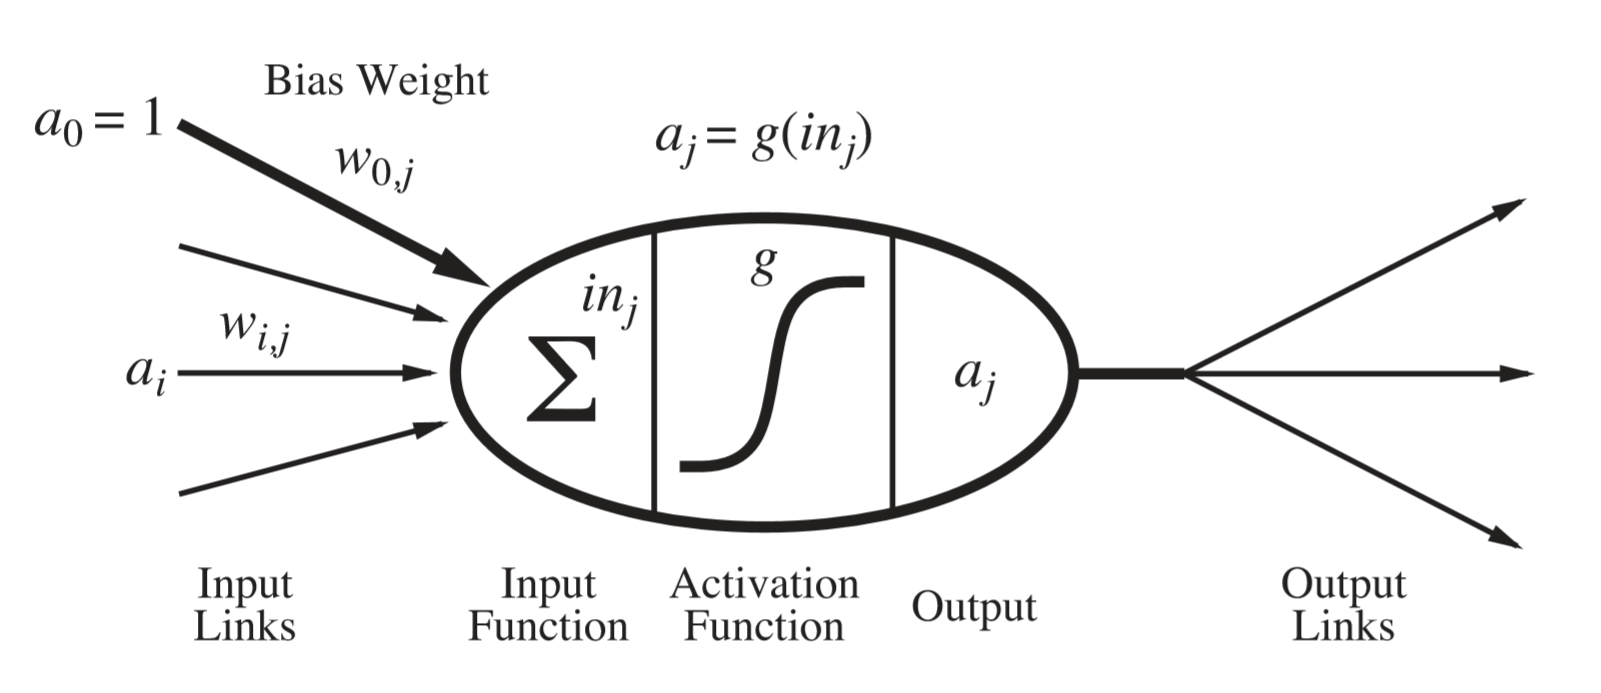
\includegraphics[width=130mm, scale = 1]{images/3_neuron.png}	
		\caption{A Simple Mathematical Neuron Representation as depicted in \cite{Russell2010}.}	
		\label{figure:Mathematical_Neuron}
	\end{figure}
	
	Figure \ref{figure:Mathematical_Neuron} shows the basic structure of a simple mathematical neuron, where the output is the result of applying an activation function to the weighted sum of inputs. The input is a collection values of $a_1, a_2, ..., a_i$.The output is a value $a_j$. Each of the inputs are multiplied by a weight $w_{i,j}$ which is a real number. The weights are important to minimize the cost of activation function and they are updated when the model is trained, through an optimization process. Often an additional term $a_0=1$ and weight $w_{0,j}=1$ are added as the bias term in the equation. Equation \ref{equation_1} represent the output after applying an activation function in the neuron showed in Figure \ref{figure:Mathematical_Neuron}.
	
	\begin{equation}
	a_j=g\Biggl(\sum_{i=0}^{n} w_{ij}\; a_i\Biggr),
	\label{equation_1}
	\end{equation}
	
	The activation function $g$ provides a way to add a non-linear relationship between the inputs and the output. Some of the functions used as activation functions are the sigmoid function, the hyperbolic tangent function, and the rectified linear unit function (RELU). \cite{Goodfellow2016}. 
	
	An alternative formulation, based on linear algebra, represents the examples as a collection of vectors $X_1, X_2, ..., X_k$. These vectors 
	are stacked horizontally on to form a matrix $X$. Next, we have the labels $Y_1, Y_2, ..., Y_k$ which are also stacked in a matrix $Y$. 
	Then the equation for the neural network becomes: 

	\begin{equation}
	Z = WX + b
	\end{equation}
	
	\begin{equation}
	Y = g(Z)
	\end{equation}

	In this formulation, $WX$ is the matrix multiplication between the examples and the weights and $b$ is the bias vector. The variable $Z$ represents the 
	result of theses operations and becomes the input to the activation function $g$ which finally yields the output of the neuron represented by the variable $Y$.
	
	\subsection{Sigmoid function}
	The {\em sigmoid function} is used to compute binary activation values in the range [0, 1]. The function is given by the following equation:

	\begin{equation}
	\sigma(Z) = \frac{1}{1 + e^{-Z}}
	\end{equation}

	The sigmoid function is interpreted as computing a probability and it is used in binary classification. Typically, an input on which the sigmoid  gives a values greater or equal to 0.5 is classified to the 1 class, whereas a values less than 0.5 is sent to the 0 class. The sigmoid function is typically used 
	in the final node of a neural network. 
	
	\subsection{Hyperbolic tangent function}
	The {\em hyperbolic tangent function} is used to compute an activation in the range [-1, 1]. and is used for activation in intermediate nodes 
	in a network. The function is given by the following equation:
	
	\begin{equation}
		tanh(Z) = \frac{e^Z - e^{-Z}}{e^Z + e^{-Z}}
	\end{equation}
	
	Typically, $tanh$  is used for activation in intermediate nodes in a network.
	
	\subsection{Rectified linear unit function}
	The {\em \ac{ReLU}}  is used to compute an activation in the range $[0, z]$, where $z$ is a real number. 
	The function is given by the following equation:
	
	\begin{equation}
	g(Z) = max(0, Z)
	\end{equation}
	
	Typically, \ac{ReLU}  is used for activation in intermediate nodes in a network. This function provides better convergence in deep neural networks. 
	
	\subsection{Softmax function}
	The {\em softmax function} is used to map a vector K with n dimension into n probability values. The formula is:
	
	\begin{equation}
	s(K_i) = \frac{e^{K_i}}{\sum_{j=1}^{n}e^{K_j}}
	\end{equation}
	
	
	Softmax is always used in the final node of a neural network used for multi-class classification. The value $s(K_i)$ represents the probability that 
	the input example belongs to class $i$. Typically, the max value of all $K_i$ is used to select the class $i$ with highest probability. 
	
	\subsection {Connecting Layers}
	To form a network, we  need to connect individual neurons as nodes in a network graph. There are many ways to build the network, but feed-forward networks are the most common ones.  Figure \ref{figure:feed-forward-network}  shows the topology of a feed-forward network. In this organization, the components are clearly separated: an input layer, an output layer and one or more hidden layers (also called processing layers). The input data is fed at
	the input layer, and the output label is  generated by the output layer. For a given neuron at layer $l$, its output is fed as input to neurons in the next layer $l + 1$. 
	
	%All connections are directed to the following layer and the internal states are just the weights themselves. The second network design the neurons have extra connections adding to a classic feed-forward network, they can be a direct recurrence when the neurons are connected to themselves,  indirect recurrence is a connection to previous layers and a lateral recurrence exist when neurons have connections with another ones at the same layer. These connections influence the neurons itself and their influence depends of the kind of recurrent design. This mean that the network is a dynamic system, the fact that this network feeds its outputs back in its own inputs permit a short-term memory, a model more seem to a brain and by the way, more difficult to understand and build \cite{Kriesel2005} \cite{Russell2010}. 
	
	\def\layersep{5cm}
	\begin {figure}[H]
	\centering
	\resizebox {\textwidth} {!} {
		\begin{tikzpicture}[shorten >=1pt,->,draw=black!100, node distance=\layersep]
		\tikzstyle{every pin edge}=[<-,shorten <=1pt]
		\tikzstyle{neuron}=[circle, fill=red!100, minimum size=20pt,inner sep=0pt]
		\tikzstyle{input neuron}=[neuron, fill=black!100];
		\tikzstyle{output neuron}=[neuron, fill=black!100];
		\tikzstyle{hidden neuron}=[neuron, fill=black!100];
		\tikzstyle{hidden1 neuron}=[neuron, fill=black!100];
		\tikzstyle{annot} = [text width=4em, text centered]
		
		% Draw the input layer nodes
		\foreach \name / \y in {1,...,3}
		\node[input neuron] (I-\name) at (0,-2*+\y) {};
		
		% Draw the hidden layer nodes
		\foreach \name / \y in {1,...,8}
		\path[yshift=0.5cm]
		node[hidden neuron] (Hb-\name) at (\layersep,-\y cm) {};
		
		\foreach \name / \y in {1,...,8}
		\path[yshift=0.5cm]
		node[hidden neuron] (H-\name) at (2*\layersep,-\y cm) {};
		
		\foreach \name / \y in {1,...,8}
		\path[yshift=0.5cm]
		node[hidden neuron] (Ha-\name) at (3*\layersep,-\y cm) {};
		
		
		% Draw the output layer node
		%\node[output neuron,pin={[pin edge={->}]right:Output}, right of=H-3] %(O) {};
		\foreach \name / \y in {1,...,2}
		\path[yshift=0.5cm]
		node[hidden neuron] (o-\name) at (4*\layersep,-3*\y cm) {};
		
		% Connect every node in the input layer with every node in the
		% hidden layer.
		\foreach \source in {1,...,3}
		\foreach \dest in {1,...,8}
		\path (I-\source) edge (Hb-\dest);
		
		\foreach \source in {1,...,8}
		\foreach \dest in {1,...,8}
		\path (Hb-\source) edge (H-\dest);
		
		\foreach \source in {1,...,8}
		\foreach \dest in {1,...,8}
		\path (H-\source) edge (Ha-\dest);
		
		% Connect every node in the hidden layer with the output layer
		\foreach \source in {1,...,8}
		\foreach \dest in {1,...,2}
		\path (Ha-\source) edge (o-\dest);
		
		% Annotate the layers
		\node[annot,above of=H-1, node distance=1.5cm] (hl) {Hidden layers};
		\node[annot,above of=I-1, node distance=3.2cm] (il) {Input layer};
		\node[annot,above of=o-1, node distance=3.2cm] {Output layer};
		\end{tikzpicture}
	}
	\caption{Feed Forward Network}
	\label{figure:feed-forward-network}
\end{figure}


\subsection{Parameters and Hyperparameters}
The {\em parameters} of a neural network model are the weights $w_{i,j}$ in each layer. Often, the notation $W^{[l]}$ is used to denote the weight matrix $W$ used at layer $l$. If we have a network with $n$ layers, then we will have $n$ weight matrices $W^{[1]}, W^{[2]}, ..., W^{[l]}, ...W^{[n]}$.  Again, the values in these matrices are called the {\em parameters} of the model. The \ac{ML} training process
involves the use an optimization algorithm that finds the right set of parameters $W^{[l]}$ for each layer $l$. These parameters are chosen as to minimize the error between the predicted label $\hat{Y}^{(i)}$ and the actual label $Y^{(i)}$ for each input example $X^{(i)}$. The most popular algorithm in used is called Gradient Descent, and has many variations such as ADAM, RMSprop, and ADADELTA \cite{Goodfellow2016}. 

In most instances, there might be multiple models to use on a given problem. In addition, multiple optimization algorithms can be tried to train a particular model. These different alternatives have impact on the training process and the parameters of the models. They are often called {\em hyperparameters} because they are not really parameters of the model, but are variables that affect training. Example hyper parameters include: a) network architecture, 
b) optimization algorithms, c) learning rate for the optimization process, and d) methods to prevent overfitting. {\em Overfitting} in a situation where the model 
works well on the training data but fails to generalize to the validation data set. 

\subsection{Data Splitting} 
The recommended procedure to find the right model involves splitting the sample data into three parts:
\begin{enumerate}
	\item {\bf Training Dataset} - this is the data used to train the network and find the parameters of the model. It is recommended to use 60\% of the data 
	for this task. 
	
	\item {\bf Validation  Dataset} -  this data is used to validate the performance of the model for a given combination of hyperparameters used for training. It is recommended to use 20\% of the data for this task. 
	
	
	\item {\bf Test Dataset} - this data is used to select the best model from a collection of models that have been trained and validated. 
	It is recommended to use 20\% of the data for this task. 
\end{enumerate} 

\section{Deep Learning with Neural Networks}

%The artificial intelligence usually solves problems intellectually challenge for the humans relatively easy, but the task the human performs easy or solve intuitively are very difficult for the computers. The problems like speech recognition or applications to find faces in images are challenge task. For these problems we must allow computers gather knowledge from the experience, avoiding specify all the knowledge that the system needs. It means build a complicated task using simpler concepts \cite{Goodfellow2016}.
%
%This approach is a \ac{ML} modern and advanced technique, the base in many advances of  \ac{AI} fields, like Natural Language Processing, Speech Recognition, Computer Vision, Biomedical Applications and so on; using the most sophisticated neural networks. 

Traditional neural networks only contain a few layers, for example: one input layer, one to three hidden layers, and a final output layer. 
Modern approaches,
however, add dozens of hidden layers with tens or even hundreds of neurons in each layer. These approaches result in models that
form complex and deep networks graphs, much more powerful  than a regular neural network. For that reason,  we know this approach as ``\ac{DL}'' \cite{Goodfellow2016,Nevala2017,Chandra2017}. Improvements in hardware, particularly Graphical Processing Units (GPU) units for massive parallel computing of neural networks,  have enable this ``deep approach". Without this technology, the computational costs to find the parameters in the deep networks would made them difficult, if not impossible, to train because they contain millions of parameters. In contrast, small 
neural networks with just a couple of layers have just a few thousand parameters and are easier to train. 

The most typical example of \ac{DL} approach is based on the feed-forward deep network. It consists in an input layer, that contains the input data for the model, next we have the hidden layers, a variable number of neurons and layers, and finally an output layer as is showed in the Figure \ref{figure:feed-forward-network}. By increasing the depth (number of hidden layers) on the network, it becomes possible to learn more complicated relationships. 
Other important methods for  \ac{DL} include the convolutional neural network (\ac{CNN}) which are used  when working with images,  and the 
recurrent neural network (\ac{RNN}),  used to process sequence data. 

\subsection{Fully Connected Networks}

Fully connected networks are the traditional feed-forward networks with many layers, as shown in Figure \ref{figure:feed-forward-network}.
Recall that for each node at layer $l$, its output is connected as input to all nodes in the next layer $l+1$.

% it means all nodes from a layer relate to all nodes of following layer and same way for the other layers. This network is a little similar to \ac{CNN} but could be computationally expensive. With modern hardware and specially using \ac{GPU} is possible achieve tasks successfully. Today we know that is not necessary to train a fully connected deep architectures due the resources that needs, but they were the first to be succeed \cite{Goodfellow2016}.

\subsection{Convolutional Neural Networks}
Convolutional neural networks (\ac{CNN}) are applied to problems with multi-dimensional data that can be represented in tensor forms (e.g, 2-D matrices, or 3-D 
cubes). For simplicity, the input of a \ac{CNN} is called an image since they are extensively used for image processing.  
The key idea in these networks is to scan the input image and apply the {\em convolution} operation between portions of the image and one {\em filter}. 
A filter is a smaller matrix $W$ which contains the parameters for the model. The operation is expressed as: 

\begin{equation}
Z = W*X + b
\end{equation}

where $X$ is the image, $W$ is the filter, $b$ is the bias vector, and $*$ is the convolution operation. Like in the case of fully-connected layers, an activation function $g$ can be applied to  the vector $Z$. In convolutional layers, \ac{ReLU} and $tanh$ are often used as activation functions. 

Each layer in a \ac{CNN} is focused in applying a convolution operation. 
There might be more than one filter in each layer, and there can be additional ``pooling layers" used to sub-sample the image and reduce its size. Current \ac{DL} approaches stack multiple convolutional layers in a row and then flatten the image to a one dimensional array. 
This array is then feed into a sequence 
of fully connected layers that end with an output layer. 

%This kind of networks is applied to problems with a grid-like topology, a clear example of this type of data are the images, other are the regular time intervals. \ac{CNN} formally is composed with a mathematical operation called convolution in at least one layer, instead of a general matrix operation \cite{Goodfellow2016}. This kind of algorithm is very used in 
\ac{CNN}s are extensively used in image processing and pattern recognition \cite{Wang2014}, as a powerful visual model to extract features in a hierarchy of concepts \cite{Long2015}. Historically this type of network was some the firsts to solve important commercial problems \cite{Goodfellow2016}, like the handwritten zip code number recognition.

\subsection{Recurrent Neural Networks}
Recurrent Neural Networks (\ac{RNN}) are networks for processing sequential data. Examples include speech recognition, language translation, and financial time series data. \ac{RNN}s are very powerful because they  efficiently store information about the past. The basic idea in a RNN is to have 
a layer of neurons that process an input data item and produces an output based on the input and a previous value from previous step. Thus, the network forms a feedback loop where the output in one time step $t$ is used in combination with the input at time step $t+1$ to produce the output for step $t+1$. In essence, the \ac{RNN} has a memory of previous events when  it produces the next output value. Like in the case of \ac{CNN}, the 
final layers of the RNN are fully-connected layers used to produce the output of the model.

\ac{RNN} are specialized to process a sequence of values \cite{Goodfellow2016}, mapping all the previous inputs to the final output. This allows the memory of old inputs to persist and influence in the next network output \cite{Graves2017}. \ac{RNN}s have also been used in image classification 
\cite{Chandra2017}. Other applications are found in the text processing: sentiment classification, topic classification, summarization, and machine translation.

%Train a \ac{RNN} for task that need information over the time is not easy, because a simple network do not maintain contextual information distant from the current step of processing. To do these kinds of task is necessary implement network more complex for maintain information as needed for future steps and remove which are not necessary \cite{Jurafsky2018}. The network more known with this type of design are \ac{LSTM} and \ac{GRU} that are described following.


\subsubsection{RNN based on Long Short-Term Memory (LSTM) }

This type of network manages the contextual information with the ability of ``forgetting" the information that is not useful and maintaining the information that has more probability to be used in next processes. Each layer has the ability to forget some previous state and give more weight to new input values. 
%The training task is specialized in achieve a better manage of contextual information to discard it or save it. 
To control the flow of information over the gates of the network, there are  specialized neural units to control how the relative weight of the current
vs the output of the previous step \cite{Jurafsky2018}. There is a forget gate that controls when  to  forget previous information and another gate to control how  much importance does the new information has.

\subsubsection{RNN based on Gated Recurrent Unit (GRU) }
\ac{GRU} is an easier way to implement a recurrent network with control of memory, and it was  is meant to be is a special case of a \ac{LSTM}. In a GRU, there is only one gate  that controls both the ability to forget about previous data and give more importance to new input values \cite{Jurafsky2018}.

\section{Natural Language Processing}
Since our goal is to find a way to measure the similarity between text in tweets, we need to briefly discuss the field of natural language processing
(\ac{NLP}). 

Basically, \ac{NLP} is the process to understand, analyze and use the human language by machines or algorithms. 
This includes  written text, voice commands, or both. The goal is to allow computers to comprehend natural language, receive 
commands, and produce results in human language. There is a lot of information contained in web pages, video sites, and social networks.   
Almost all of it is
written or recorded in natural language, and that is a major  reason why we want our algorithms to understand human language, in  oder   to acquire 
all this information from written and spoken language. A \ac{ML} model that wants to acquire knowledge needs to comprehend at least partially the  use of human language  (e.g. ambiguity and messiness). This undertaking is not trivial because the presence of the colloquialism, figure of speech, abbreviations and emoticons, to mention a few \cite{Russell2010,Nevala2017} . The difference with a computer language (e.g. python or java) is that a natural language cannot be characterized in a set of sentences, because they are very large, ambiguous, and constantly changing;  in the state-of-the art models
models are just an approximation \cite{Russell2010}.

The process of language analysis is closely related to linguistic, traditionally, this process is decomposed in three stages: syntax, semantic and pragmatics. We first analyze the syntax of a text providing an order and a structure, then  analyze  the text in terms of meaning (semantic), and the last stage is a pragmatic analysis, which relates the sentence with a context. Such separations constitute the basis for structural models from a software point of view, making the analysis more manageable and serving as a starting point. Recently, deep learning solutions are not focused on this scheme and they try to understand language straight from the raw data examples \cite{Indurkhya2010}.

\begin{figure}[H]	
	\centering
	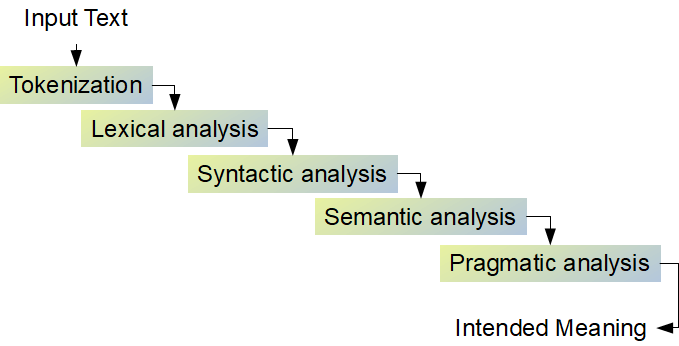
\includegraphics[width=100mm, scale = 1]{images/4_nlp.png}	
	\caption{Natural Language Process Stages}	
	\label{figure:NLP_Stages}
\end{figure}

Figure \ref{figure:NLP_Stages} represent the stages in a  traditional \ac{NLP} pipeline. The first step, tokenization,  divides a continuous text  into words or sentences. In English, text is usually separated by whitespaces but other unsegmented languages are more difficult because there is not a visible separation between words (e.g. Chinese, Japanese). The second stage is lexical analysis, which refers to morphological processing, mapping strings to lemma and assigning structure to words, and registering their structural properties. The third stage is syntactic analysis where a sentence is processed to determine its structural composition, following rules of a formal grammar to finally assign a meaning to the sentence. The syntax tree is the standard to represent a syntactic structure which contains the steps in the derivation from the initial sentence. The fourth stage is semantic analysis, and it is related with the context of words, phrases, etc. This stage not only refers to the meaning of a sentence, but also to its relationship with other words or sentences, to infer meaning of the text. The final stage is pragmatic analysis, also called natural language generation, and  it is the process when a machine can understand natural language as input and produce natural language as output with the intention to communicate something with a correct context \cite{ Indurkhya2010}.

Applications of \ac{NLP} are based on probability distributions over sequential data in a natural language. We can use generic neural networks for basic tasks, however, in complex applications, we need specialized techniques to process data, sometimes like a sequence of words, characters or even bytes. The earliest successful language model, a probability distribution over sequential data, was n-gram models (sequences of tokens). It has many possible types: unigrams, bigram, trigram, n-gram. In order to improve statistical efficiency, researchers introduced the notion of word categories or class-based n-grams models; however these models are not able to share statistical strength of similar words and their contexts. 

Neural network  models have been able to recognize the similarity not only between words but also in their contexts and how words are distributed with each other. This word representation sometimes is called  distributed representation or word embedding, which means that language symbols are represented as points in a multi-dimensional vector space . In an embedding space, words with similar meaning are close to each other \cite{Russell2010,Goodfellow2016} because they are represented by vectors that are close by in the vector space (in the Euclidean distance sense). The best known word representation are Word2Vec Models \cite{Mikolov2013}, an improved of skip-gram model in terms of quality of vectors, and speed training \cite{Mikolov2013} and GloVe model that combines the advantages of global matrix factorization and local context window \cite{Pennington2014}. More recent studies show other sentences encoder like Skip-Thought Vectors, an approach for unsupervised learning that tries to reconstruct passages of text that share semantic properties \cite{Kiros2015}. There is also the  Supervised Learning of Universal Sentence Representations from Natural Language Inference Data, an encoder using pre-trained sentence level embedding with supervised data of Stanford Natural Language Inference datasets demonstrating stronger transfer task than skip-thought vectors \cite{ Conneau2017}. Also, we have the Universal Sentence Encoder, which uses supervised data to train a sentence embedding model instead of a word level embedding, showing a good performance \cite{Cer2018}. 

There are several important applications of \ac{DL} techniques in \ac{NLP} tasks including:

\begin{itemize}[nolistsep]
	\item \textbf{Spelling and Grammar Checking:} The suggestions that appear when we type a text in a smartphone or when we redact a document in an advance text editor. 
	
	\item \textbf{Text Classification:} It is the categorization of a text in a defined set of classes (e.g., hate speech), or the language identification, or the  spam detection in email messages \cite{Russell2010}.
	
	\item \textbf{Information Retrieval:} Search, retrieval, and ranking  of documents responding to a keyword query.
	
	\item \textbf{Summarization:} Automatic generation of  the essential information from a long document into a shorter piece of text.
	
	\item \textbf{Syntactic Analysis:} The analysis of a string of words to isolate subjects, verbs, adverbs, adjectives, and others complements (phrase structure) \cite{Russell2010}.
	
	\item \textbf{Machine Translation:} It is the task to automatic translation of a sentence into an equivalent sentence in meaning in another natural language \cite{Goodfellow2016}.
	
	\item \textbf{Speech Recognition:} This task identifies the words spoken to determine their meaning. That is difficult because the ambiguity and noise are a hard challenge \cite{Russell2010}.
	
\end{itemize}

\section{Text Similarity}
{\em Text similarity} refers to how close is a piece of text $T_1$ to another one $T_2$ in terms of meaning and structure.  The first means semantic similarity and the last is called lexical similarity. All works in lexical similarity often are developed to achieve semantic similarity \cite{Ganesan2015}.  Lexical similarity exists when there is character or word matching (e.g. ``feel'' and ``feet''). On other hand, semantic similarity is based on meaning and context (e.g. ``President of the United States' and ``POTUS") \cite{Pradhan2015}. 
Text similarity is used in many \ac{NLP} problems such as text classification, clustering, information retrieval, topic detection, machine translation, summarization and others \cite{Pradhan2015,Majumder2016}, \cite{Gomaa2013}. It is used heavily in research related with social network analysis \cite{Zhang2015}.  

\subsection{Lexical Similarity}
Lexical similarity refers to structurally similar words or characters in the evaluation sentences (matching or comparison). 
%Hence in this kind of similarity, the meaning is not known then we can use lexical analysis techniques to achieve better accuracy, for example we can add no-determiner words to expand the scope and provide some of context \cite{Ganesan2015} \cite{Gomaa2013}. This metric could be used on clustering, redundancy removal and information retrieval \cite{Ganesan2015}. 
Lexical similarity could categorize text depending of the granularity used. It can be character level, word level, or phrase level \cite{Ganesan2015,Pradhan2015}. String-based methods to calculate the measure of similarity are categorized as follows:

\begin{itemize}[nolistsep]
	\item \textbf{Character based similarity:} There are many techniques  based on characters. The longest common substring/subsequence is a method that finds substrings and compares them based on a common chain of characters they both share. This is the longest common chain of suffixes for each substring. Another idea is the Levenshtein distance, where the similarity measure is given by the number of operations to transform one string in another one, using insertions, deletion or substitution of adjacent characters. The Jaro distance is another method that emphasizes in the number and order of matching common characters; it is used in duplicate detection (record linkage). Finally, the n-gram method  calculates the distance of two sub sequences, dividing its similar n-grams by maximal number of n-grams. \cite{Pradhan2015,Majumder2016,Gomaa2013}.
	\item \textbf{Statement/Term based similarity:} A method widely known in text similarity is cosine similarity, where the similarity distance is given by the cosine of the angle between two vectors in an inner product space. These vectors represent the sentences being considered. Euclidean distance, also called L2 distance, use vectors in a Euclidean space where the distance is the square root of the sum of squared difference between two vectors (sentences). Jaccard similarity coefficient or Jaccard index is used to calculate similarity and diversity in sets; it takes the shared term in the intersection and divides it by the number of all terms of the union. There are other known methods like block distance (Manhattan distance, L1 distance, etc.), Dice's Coefficient, Matching coefficient, overlap coefficient, soft-cosine similarity and centroid based similarity, among others \cite{Pradhan2015,Majumder2016,Gomaa2013}.
\end{itemize}

\subsection{Semantic Similarity} \label{sem_sim}
Semantic analysis entails a deeper level of analysis, including the meaning and the context of sentences. For example syntactic parsing to get dependency structure in the phrases. Commonly semantic similarity use background information about concepts like WordNet, or Wikipedia,  or a simplify corpora of texts  \cite{Ganesan2015,Zhang2015}.
Semantic similarity is frequently used for text summarization, topic analysis, recommendation system, and collaborative tagging system, among others. This approach could be classified in three big categories based in the use of information: corpus based,  knowledge based and hybrid methods \cite{Gomaa2013, Zhang2015}, described below.

\begin{itemize}[nolistsep]
	\item \textbf{Corpus based similarity:} 
	Also called statistical similarity, this approach refers to the use  of information gathered from a large corpus from written o spoken data. Latent semantic analysis represents the text in a matrix where rows are the unique words and columns represent each sentence. This method is constructed based in a corpus of text and a mathematical technique called singular value decomposition to reduce dimensionality while maintaining similarity relation between word and text. To calculate the similarity is often used cosine similarity.  Another technique is hyperspace analogue to language, a variation of latent semantic analysis, taken a set of words called a ``window'', and is compared with the corpus to calculate co-occurrences in words, forming a matrix representing the strength between related words. Its similarity also can measure with cosine similarity method. Explicit semantic analysis uses the Wikipedia corpus to convert sentences in a tf-idf (term-frequency-inverse document frequency) weighted vector between each word and the documents of corpus. The measure to calculate the distance between vector is cosine similarity. Normalize Google distance is a semantic metric that uses Google search to get the number of hits returned for each term of the text and build a metric to calculate the words with similar meaning between two sentences. Other methods are point wise mutual information, normalized information distance, and normalize compression distance  \cite{Ganesan2015,Majumder2016,Gomaa2013,Zhang2015}.
	
	\item \textbf{Knowledge based similarity:} It is called topological similarity and it is based in semantic networks; these networks are a lexical database grouped in set of semantic synonyms with conceptual and lexical relations that include verbs, nouns, adverbs, and adjectives. The most popular semantic networks are Word Net and Natural Language Toolkit \cite{Pradhan2015,Majumder2016,Gomaa2013}. There are distinct types of categorization focused in similarity or relatedness. The node-based (also called information content based) similarity that calculates the similarity between two sentences by the amount of information that share each other; Resnik similarity method uses only Word Net nouns to get the information content of sentences; other measures are Lin method, Jiang and Conrath method \cite{Pradhan2015,Majumder2016,Zhang2015}. Edge-based approach counts the edges of graphs (semantic network) between the compared concept nodes where nodes with shorter path are more similar. All edges are weighted considering network density, node depth, type of link, and link strength \cite{Majumder2016,Zhang2015}. Other approach is feature-based, which uses the concepts of Word Net as a list of features to calculate the semantic similarity between sentences \cite{Zhang2015}, and finally gloss-based approach uses glosses of words from a given corpus; Vector Measure is a method that forms a co-occurrence matrix with the average of each co-occurrences vector of a gloss/concept to measure the semantic similarity \cite{Pradhan2015,Zhang2015}.
	
	\item \textbf{Hybrid similarity measures:} This approach is a combination of many features, like lexical structure and corpus information, combining several metrics into one. For example, semantic text similarity method is a combination of syntactic and semantic information \cite{Gomaa2013,Zhang2015}. Other methods combine more approaches, according to \cite{Zhu2014} which built a supervised random forest regression model that use machine learning methods to combine string features, corpus-based methods, knowledge-based methods, syntactic features, and multi-level text features.
	
\end{itemize}

\chapter{Problem Formulation} \label{chapter 3}
\section{Description}
Our work is rooted in \ac{THS} project at UPRM, whose goal is to monitor tweets related to medical conditions, and detect instances where
a disease is actively being discussed in a given region.
The main problem that we want to tackle in this project is the development of  \ac{DL} models that can evaluate the similarity between
tweets. Specifically, given an example tweet $T_p$ and a collection of tweets $T_1, T_2, ..., T_n$, we want to rank the collection of tweets
from the most similar to the least one to $T_p$. In order to do, {\bf we need to develop a method to measure the similarity between pairs of 
	tweets}. Our goal is to use \ac{DL} to achieve this. 

First, we need to create a collection of labeled tweets to help us determine how humans 
view similarity. In this collection, we have rows with triplets $(T_p, T_{h_1}, T_{h_2})$, each element being a tweet. For each row, the first tweet, $T_p$ is the ``example" tweet called the ``premise". Next to it, we have two additional tweets, $T_{h_1}, T_{h_2}$, called the
hypothesis tweets. Users are asked to compare the premise with each of the two hypothesis tweets, and rank which one is more similar to the 
premise. This is done by providing a numeric value on their similarity. The value is in the range (0,4), with 0 being unrelated tweets and 4 being identical in term of meaning. Thus, for example, if the rank between $T_p$ and  $T_{h_1}$ is 1, and the rank between $T_p$ and  $T_{h_2}$ is 3, then 
tweet $T_{h_2}$ is more similar to $T_p$.

With this labeled data set, we then aim to train a model than can learn to do this ranking and learn how to give a similarity score between 
the example tweet $T_p$ and another tweet $T_i$ that we want to consider. Our approach borrows ideas from the work in \cite{Wang2014} which find  similarity between images. 

By using a \ac{DL} model trained to rank tweets based on similarity, users could: 
\begin{itemize}
	\item pick a tweet - the example tweet- that they consider useful for detecting conversations about a given disease and
	\item setup a process to watch the Twitter stream, collect tweets similar  to the example one, and visualize these tweets  sorted by 
	relevance of their similarity. The model can be used to compute a similarity score between the example tweets and each tweet read from the stream. Then, sorting can be used to provide a ranked list based on the similarity.
\end{itemize} 

As we described in section \ref{sem_sim},   text similarity measures are very difficult to calculate  because it is hard to find the meaning and context match of the two pieces of text. To manage those issues, we use relevant information to find context similarity and syntactical similarity, like the type of disease mentioned in each tweet,  or if the tweet is related to a disease or not. This contextual information can be used as pre-processing step before feeding 
the tweets to the \ac{DL} model.

% and a metric that describe the level of similarity between tweet texts, that are tagged in a range of one to four, where one is less similar and four is more semantically similar.

\subsection{Examples}
We now provide some examples of tweets to show the complexity of working with data related to semantic measures and contextual similarity.
We obtained these tweets form the actual Twitter stream.

\begin{definition} {\bf : Tweets that are not related and discuss different diseases.}
	\begin{itemize}[nolistsep]
		\item Measles starts with cold like symptoms that develop about of days after becoming infected this is followed a few days later by the measles rash poster shows us the symptoms to look out for think measles prevention is best a dose of vaccine needed vaccines work.
		\item The Ebola outbreak was a worst nightmare for countries affected interestingly Ebola was not a new disease in fact on managing the disease there is a forty year old knowledge so how did Ebola become such an epidemic.
	\end{itemize}
\end{definition}

In this example, the two tweets discuss about diseases. The first one of them describes the symptoms of measles, and recommends vaccines as the method
for  prevention. The second tweet does a question about the reason why Ebola has expanded if this disease is not new and there is enough knowledge about it. The content of these two tweets are related with a health condition but they are describing different diseases, that is enough to consider them not similar.

\begin{definition} {\bf : Tweets that are not related and discuss the same disease}
	\begin{itemize}[nolistsep]
		\item Theory man flu exists as a phenomenon because it is the only time toxic masculinity tells men it is okay to feel vulnerable weak and look to their partners for support.
		\item Yeah, I missed like a day of school on and off flu I could not even eat, and I could not walk without feeling like vomiting or collapsing.
	\end{itemize}
\end{definition}

The first tweet refers to the flu, but it is not about a health condition. It discuss  an assumption about how the flu exists to show the vulnerability of weak  men. The  other tweet is discussing about someone that missed a school day because flu and describes  his/her symptoms.


\begin{definition} {\bf : Tweets that are  related  and discuss the same disease}
	\begin{itemize}[nolistsep]
		\item I wish I knew if the twins were going to get the flu like what is the usual window, he is had it symptom wise since Sunday night and it is Tuesday so when would they likely show symptoms ahh.
		\item So I was at the hospital and obviously could not type while I was there since, a I could not type and b I was scared of being caught with lewd rps after I healed bad luck struck again and I was bedridden with the flu all I did was sleep and I was coughing so much my eyes went red.
	\end{itemize}
\end{definition}

In this case the first tweet mentions to twins getting flu and describe the intervals of days with possible symptoms. The second tweet is about a person who was in the hospital and explains that was the reason because he could not type, and when he was recuperated, then he got flu again and just goes to sleep. The two sentences are showing a health condition (flu) where the writers are explaining symptoms and what they were doing when they got flu. Therefore, these tweets are related.

\section{Formalization}\label{formalization_problem}
We are now in a position to better formalize the problem at hand, considering a premise tweet $T_p$ and a collection of tweets 
$T_1, T_2,..., T_n$. Let $diff(T_i, T_j)$ be a function that computes the similarity between  two tweets $T_i$ and $T_j$ as their distance 
in some n-dimensional embedding (vector) space. The smaller the value for $diff()$, the more similar are $T_i$ and $T_j$.   Let $rank(T_i, T_j)$ be a function that assigns a comparison rank to $T_i$ and $T_j$ in the range (0,4); the closer to the value 4, the more similar are $T_i$ and $T_j$.
We define the following property for $rank(T_i, T_j)$:

\begin{property}{\bf Rank Property}\\ 
	Given three tweets $T_p, T_{h_1}, T_{h_2}$, if $rank(T_p, T_{h_1}) > rank(T_p, T_{h_2})$ then $diff(T_p, T_{h_1}) < diff(T_p, T_{h_2})$.
\end{property}

With this property we establish the $rank()$ as an alternative method to measure similarity. The higher the rank  the more similar the tweets. 
Our goal is then train a model $M$ to compute the function $rank(T_i, T_j)$.

Notice that the $diff()$ function is an unbiased measure of similarity, but it is difficult to find a general similarity metric, as discussed in 
Chapter \ref{chapter 2}. Instead, our $rank()$ function
tries to approximate human ability to make the comparison and establish similarity. 

%The goal in this project is classify if a tweet is similar to another from a stream of tweets $S = {s_!, s_2, … , s_n}$. Our model is a supervised approach, where the target keywords are associated with a disease group $G = {g_1, g_2, …, g_n}$. G is conforming by five diseases \textit{flu, measles, zika, diarrhea and Ebola}.

\subsection{Scope of the Model}
\ac{ML} models are bound to work on data coming from the same distribution as the data for training. In order to properly scope our model, we limit the data set to include tweets that contain the following medical keywords:

\begin{itemize}[nolistsep]
	\item Flu
	\item Zika
	\item Ebola
	\item Measles
	\item Diarrhea  
\end{itemize}

Sometimes, the keywords mentioned above are used in colloquial conversations that are not related with medical 
issues, which can mislead researchers into believing the occurrence of a keyword implies a disease outbreak. 
For that reason, the tweets are then organized and labeled in three classes:
%The belong to a medical condition is given by a manual classification of tweets into the next three classes:

\begin{itemize}[nolistsep]
	\item \textbf{0}: Tweet does not belong to a medical condition.
	\item  \textbf{1}: Tweet belong to a medical condition.
	\item \textbf{2}: Tweet has an ambiguous meaning, it is difficult to classify 
\end{itemize}

Clearly, in a production setting, we are only interested in working with tweets that belong to class 1. 

\subsection{Use in Production}
Once the model $M$ is trained, we want to use it in the production task following these steps:

\begin{enumerate}
	\item Subscribe to the Twitter data stream to build a collection ${\bf T} = \{T_1, T_2, ..., T_n\}$.
	\item Chose a premise tweet $T_p$.
	\item Compute the $rank(T_p, T_i) $ for each tweet $T_i \in {\bf T}$, and store the triplet $(T_p, T_i, rank(T_p, T_i))$.
	\item Sort the triplets $(T_p, T_i, rank(T_p, T_i))$ in decreasing rank order.
\end{enumerate}

With this procedure, the tweets more similar to $T_p$ are sorted from most similar to least similar.

%The last target is a measure of similarity between a pair of tweets in range of one and four. The complete description of how is taken this measure is given in section \ref{define_similarity}
%
%We apply pre-processing and \ac{NLP} tools over tweets to filter and select whatsoever related to a medical condition, and built triplets taking only tweets with labels 1 or 0. Let us call the result of this process S'. Now we apply a classifier $\hat{y}$ in a triplet $s' \in S'$ to classify the pair of tweets in the triplet that are more similar. After training $\hat{y}$ classifier, it can be used as long data come from the same source. If we change G elements, we must be retraining the algorithm with the new keywords present in G.
%
%The distribution of samples respect to belonging to a medical condition or no, are not uniform, with class 1 being majority. In this case we are dealing with a class imbalance problem \cite{Batista2004} \cite{He2009}. To tackle this problem, we use a penalty technique during training task, a higher penalty is given when occur a wrong classify of a sample that belongs to the minority class.

\section{Data Processing Architecture}

\begin{figure}[H]	
	\centering
	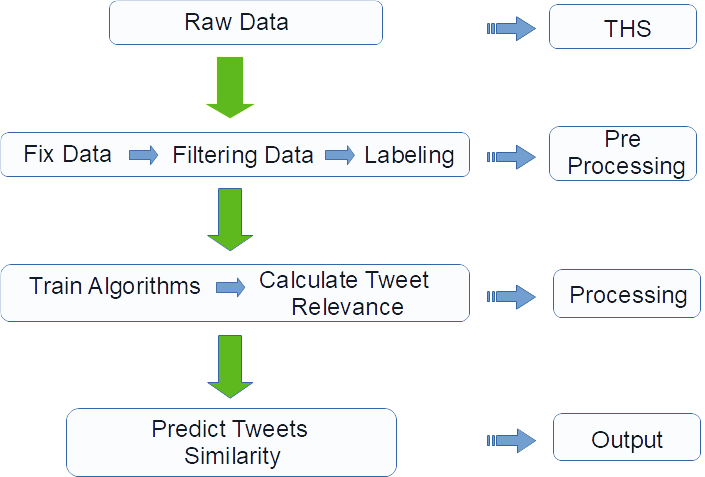
\includegraphics[width=110mm, scale = 1]{images/5_data_processing.png}	
	\caption{Data Processing Architecture}	
	\label{figure:data_processing}
\end{figure}

Figure \ref{figure:data_processing} depicts the architecture for 
tweet processing that we shall implement to train and use in our models. The architecture is based in the THS system \cite{8029348, 8622504}.
Tweets are collected in  the \ac{THS} system and stored in a distributed database system (Hive)  using \ac{HDFS}. Tweets are ``cleaned'', removing links, hashtags and mentions.  
%In a next stage the text passes through a pre-processing expanding contractions and correcting misspelling.
In the next stage, tweets are filtered and associated to a disease. After detecting if the text is related to a disease, tweets are labeled to determine if each tweet is discussing about a disease or if it is a lexical or semantical ambiguity. This is done using the model trained in \cite{8622504}. 
In order to train the similarity model, triplets of tweets are given to human labelers so they can provide a score of similarity between the 
first tweet (premise) and the other two tweets (the hypotheses). 
%Other process to prepare the data to training is take an average measure of three labelers about the level of similarity between tweets as part of pre-processing stage.
Once the similarity model is trained, it can be used by the production model for find the similarity of tweets.

%The previous stages are the input of the main process to train algorithms and calculate tweets relevance and after to present these tweets to the user sorted by relevance of their similarity as the output of the model.

\chapter{System Architecture and Organization} \label{chapter 4}
\section{THS System Overview} \label{ths_system}

\ac{THS} is a collection of Big Data tools running on a cluster system at \ac{UPRM} to collect, filter, and store the tweet data to future uses. We use \ac{ML} tools to process data; such as  Keras \cite{Keras2019}, TensorFlow \cite{Tensor2019}, Scikit-learn, and others. Our current \ac{THS} system consists of 12 nodes in a big data environment, organized as follows: One master-node, one client-node, and 10 data-nodes. The big data tools installed are \ac{HDFS} \cite{Hadoop2019}, \ac{YARN} \cite{Hadoop2019}, Apache Kafka \cite{Kafka2019}, Apache Spark \cite{Spark2019}, and Apache Hive \cite{Hive2019}.

The data processing pipeline is shown in Figure \ref{figure:ths_system} and detailed step by step as follows:

\begin{itemize}
	\item \textbf{Step 1:} We subscribe to the Twitter \ac{API} to save raw tweet data, building a real-time data stream using Kafka, a distributed streaming platform \cite{Kafka2019}. The script (``producer.py'') runs on the edge-node (client-node) of our cluster identified as node05.ece.uprm.edu. In this step, we filter data by language (e.g. English) and by keywords of target medical diseases (e.g. Flu, Measles). The purpose of this script is to keep with  the Twitter stream, collecting data, and 
	passing it down the pipeline for its eventual processing.
	
	\item \textbf{Step 2:} All raw data obtained from the Twitter \ac{API} is stored in the Kafka pipeline for later processing. Each stored record consists of a key, the data, and a timestamp. Kafka is configured to keep data for 3 hours; after that time, the system discards raw data automatically to save disk space. 
	
	\item \textbf{Step 3:} In another script called ``consumer.py'' we connect to a stream ``topic'' in Kafka to get tweets  by arrival order. This script is in turn  connected to 
	the Apache Spark streaming system. The purpose of this script is to remove the data from the Kafka queue for processing. Thus, the producer and consumer
	scripts implement an asynchronous	data pulling pipeline. 
	
	\item \textbf{Step 4:} The Spark streaming system collects the data from the consumer and begins to clean data, filtering and keeping only real tweets, and discarding re-tweets or replies. %Making use of spark tools we create ``data frame'' to process, manage and save data in a Hive database.
	
	\item \textbf{Step 5:} Data is saved in Hive tables at regular time intervals with specific information that include users, keywords, hashtags, geolocation, and the original raw tweet. This data is used to future processes and searches.
	
	\item \textbf{Step 6:} Data stored in Hive database is used to generate data visualizations and, in this project, to get data samples to train a  neural network models to measure the similarity between tweets.
	
\end{itemize}

\begin{figure}[H]	
	\centering
	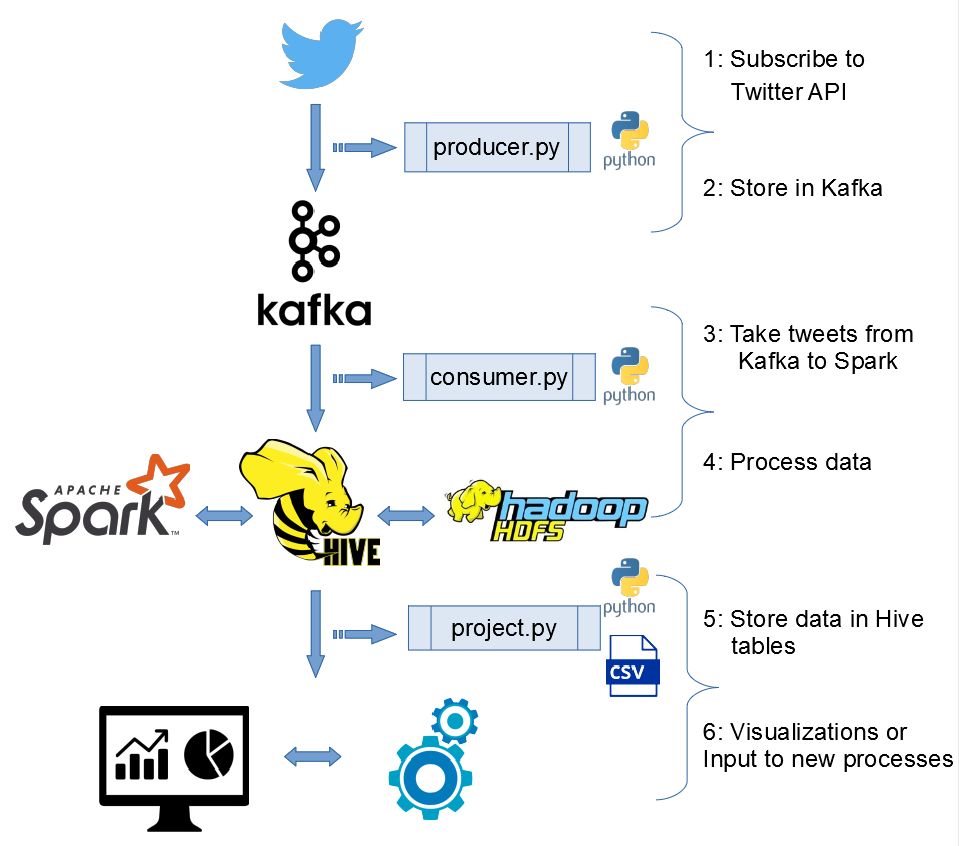
\includegraphics[width=150mm, scale = 1]{images/6_ths_system.png}	
	\caption{\ac{THS} Processing Architecture}	
	\label{figure:ths_system}
\end{figure}

\section{Strategy to Obtain the Model for Similarity \label{strategy}}
In order to obtain a model $M$ that can compute the similarity rank between two tweets, we follow the strategy in \cite{Wang2014}, and first train a bigger model $M'$
that is capable of classifying relative similarity in triplets of tweets. This is a common strategy in \ac{DL}: {\em train a bigger model that does a task in which the model you really want is  
	a sub-task (sub-model)}. This is done because the bigger model might be easier to train on its intended task, or because there is data already available to train the bigger model.  Once the bigger model is trained, the sub-model is taken out and used in standalone fashion. In our specific case, the task that performs model $M$, computing the similarity between two tweets, becomes a sub-task in a bigger
model $M'$. In this case, $M'$ receives a triplet $(T_p, T_{h_1}, T_{h_2})$ and emits a classification value as follows: 

\begin{itemize}
	\item 0 - tweet $T_{h_1}$ is more similar to $T_p$ than is tweet $T_{h_2}$.
	\item 1 - tweet $T_{h_2}$ is more similar to $T_p$ than is tweet $T_{h_1}$.
\end{itemize}

In order to train $M'$, {\em we need to first compute the similarity between pairs of tweets}, and this is exactly what model $M$ will do. But it is much easier to ask humans to establish a rank between three tweets, as opposed to ranking many more tweets and trying to compare just two of them. The authors in \cite{Wang2014} used this same idea but for 
the case of computing image similarity. Our approach is to make make $M$ part of $M'$, 
train $M'$, and then extract the sub-components in $M'$ that belong to $M$. 

\section{Labeling}
In order to work with the strategy presented in section \ref{strategy}, we created a data set for labeling. 
The dataset consisted of  4,225 triplets $(T_p, T_{h_1}, T_{h_2})$. All the tweets in these triplets were known to 
be related with a medical conditions, and had one of the five target keywords: Ebola, Zika, Flu, Measles, or Diarrhea.
There were 54 labelers, which were students from UPRM
that were enrolled in the course ``Introduction to Database Systems". Labelers were instructed to:
\begin{itemize}[nolistsep]
	\item compare $T_p$ with   $T_{h_1}$ and  $T_{h_2}$,
	\item rank the similarity between $T_p$  and   $T_{h_1}$ on a scale in the range (1,4), and
	\item rank the similarity between $T_p$  and   $T_{h_2}$ on a scale in the range (1,4).
\end{itemize}

\section{Building the Dataset for Training \label{buildtrain}}
In all of our data sets, the first tweet in the triplet , $T_p$, is always related with a disease. 
We took the data set from the previous section, and augmented it by adding two additional group of triplets.  In the first group, one of the 
hypothesis tweet, $T_{h_i}$ has the same disease keyword as $T_p$ but is not related with a medical condition (class 0). In this case, the 
ranking of this tweet with respect to $T_p$ is set to 0. In the second group, one of the hypothesis tweet, $T_{h_i}$ has a different disease keyword as that $T_p$.  In this case, the ranking of this tweet with respect to $T_p$ is also set to 0. In total, we grew the training data set to 11,425 tweets. 

The next step was to prepare the data and align it according to the model that we wanted to train. We took every triplet $(T_p, T_{h_1}, T_{h_2})$
and converted into corresponding tuples (a finite ordered list of elements) of the following shape:

\[
(T_p, D_{T_p}, M_{T_p}, T_{h_1}, D_{T_{h_1}}, M_{T_{h_1}},T_{h_2}, D_{T_{h_2}}, M_{T_{h_2}}, rank(T_p, T_{h_1}), rank(T_p, T_{h_2}), L)
\]
The structure of these tuples is as follows:
\begin{itemize}
	\item $T_p$ - premise tweet.
	\item $D_{T_p}$ - index for the medical condition in $T_p$. Indices used: 0 - Flu , 1 - Ebola , 2 - Measles  , 3 - Diarrhea, 4 - Zika. 
	\item  $M_{T_p}$ - classification label of the tweet $T_p$: 0 - not related with a medical condition, 1 - related with a medical condition, 2 - ambiguous. 
	\item $T_{h_1}$ - first hypothesis tweet.
	\item $D_{T_{h_1}}$ - index for the medical condition in $T_{h_1}$. Indices used: 0 - Flu , 1 - Ebola , 2 - Measles  , 3 - Diarrhea, 4 - Zika. 
	\item  $M_{T_{h_1}}$ - classification label of the tweet  $T_{h_1}$: 0 - not related with a medical condition, 1 - related with a medical condition, 2 - ambiguous. 
	\item $T_{h_2}$ - second hypothesis tweet.
	\item $D_{T_{h_2}}$ - index for the medical condition in $T_{h_2}$. Indices used: 0 - Flu , 1 - Ebola , 2 - Measles  , 3 - Diarrhea, 4 - Zika. 
	\item  $M_{T_{h_2}}$ - classification label of the tweet $T_{h_2}$: 0 - not related with a medical condition, 1 - related with a medical condition, 2 - ambiguous. 
	\item $rank(T_p, T_{h_1})$ - similarity ranking between $T_p$ and  $T_{h_1}$ as given by the labelers.
	\item $rank(T_p, T_{h_2})$ - similarity ranking between $T_p$ and  $T_{h_2}$ as given by the labelers.
	\item $L$ -  classification label for relative comparison between tweets: 1 - if $rank(T_p, T_{h_1}) >= rank(T_p, T_{h_2})$, 0 - if  $rank(T_p, T_{h_1}) < rank(T_p, T_{h_2})$.
	
\end{itemize}
%\section{How to Define Similarity}\label{define_similarity}
%
%The measure of similarity is represented by one (1) or zero (0). Its value depends of the relevance measures of triplets (group of three tweets). The measure of similarity is defined in the following function.
%
%\begin{equation}
%s(t_0, t_1, t_2) = 
%	\begin{cases} 
%		1 		& \text{if } r(t_0, t_1) \geq r(t_0, t_2) \\	
%		0 		& \text{if } r(t_0, t_1) < r(t_0, t_2)
%	\end{cases}
%\end{equation}
%
%\noindent Let $s(t_0, t_1, t_2)$ represent the similarity between  tweets in a triplet, when  $r(t_0, t_1) \geq r(t_0,t_2)$ is true then the value is 1, and when $r(t_0, t_1) < r(t_0,t_2)$ the value is 0; this means 1 if  $t_0$ is more similar to $t_1$ than it to $t_2$ and  0  if $t_0$ is more similar to $t_2$ than it to $t_1$.
%
%\begin{equation}
%r(t_i, t_j) = \sum^n_{k=1} \frac{m_k(t_i, t_j)}{n}, \text{where } m_k(t_i,t_j) \in \mathbb{N}, 1 \leq m(t_i,t_2) \leq 4
%\end{equation}
%
%\noindent The function of relevance $r(t_i, t_j)$ is calculated by two ways. The first way is estimated automatically because tweets have a marked difference in meaning, considering the disease class and their label value. In other hand when the value labels are calculated manually, the relevance is the average of sum each relevance measure of the pair of tweets, where the measure of relevance can take a value in a range of 1 to 4, depending of level of relevance of similarity. To higher value means more similarity between them. The process to labeling the relevance level and similarity of triplets are described in section \ref{data_relevance_labeling}

\section{Architecture of the Learning Model}\label{models}
The tuples described in the previous section are used in our method, and we train a model $M'$ on the following {\em classification task}: 
{\bf determine which tweet is more similar to $T_p$} : 
$T_{h_1}$ or $T_{h_2}$. In doing so, we will be training a sub-model $M$ that does a {\em regression task}: compute the $rank(T_p, T_{h_i})$ between the 
premise and a hypothesis. $M$ {\bf will become the model that is actually used in production to rank tweets}. 
Our approach  is a novel adaptation of a triplet-based network architecture \cite {Wang2014}, modified to classify if tweets are similar or not. It is based on the level of similarity between tweets and their relatedness with a disease.  
The input to train the algorithm is given in a \ac{CSV} file that contains tweets and its label values (see section \ref{data_labeling}) in the tuple form presented in section \ref{buildtrain}. Input data passes through a process to finally obtain the measure of similarity between a pair of tweets. 

%The entire process is shown in Figure \ref{figure:all_model}.

Figure \ref{figure:all_model} depicts the organization of the \ac{DL} model that we used.
The  model starts with an embedding layer. Each of the tweets in a tuple passes through an embedding process to convert sentences into a matrix of multidimensional vectors, each row representing words. This embedding layer is a modified siamese network since it is the same layer and weights are 
used to compute the embedding of the premise tweet $T_p$ and hypothesis tweets $T_{h_1}$ and $T_{h_2}$.  Next, we have the Combiner Layer, where we use different approaches such \ac{RNN} and \ac{CNN} to extract 
features from the data.
We use  several combinations of hyperparameters until we get better results.

In the relevance layer we add a second input, called auxiliary input, that contains the information about the medical keyword of the tweet and the label indicating if the tweet is actually related with the medical condition or not. Again, we use the siamese network concept to pass this information for each tweet in the input.
Using the auxiliary input and the output of the Combiner Layer, we calculate the relevance between the premise tweet and hypothesis tweet. This value becomes the rank of the premise and hypothesis. 

Up to this point, the neural network has trained $M$, the model that computes the similarity ranking and the one we
actually want in production. But  the process
is not finished.
The final network component is the classification layer that is composed of a sequence of dense layers that end with a sigmoid classifier to finally get an output with value of zero or one. A label of  1 means that the first hypothesis  $T_{h_1}$ is more similar to the premise $T_p$ , and 0 means that the second hypothesis
$T_{h_2}$ is more similar to the premise $T_p$. This neural network is model $M'$ that we have referred as the ``bigger" model to be trained. Notice how 
training $M'$ indirectly trains model $M$, since we need to have the similarity ranks in order to make the comparison between $T_p, T_{h_1}$ and $T_{h_2}$, and emit the final label of the classification task. 

\begin{figure}[htbp]	
	\centering
	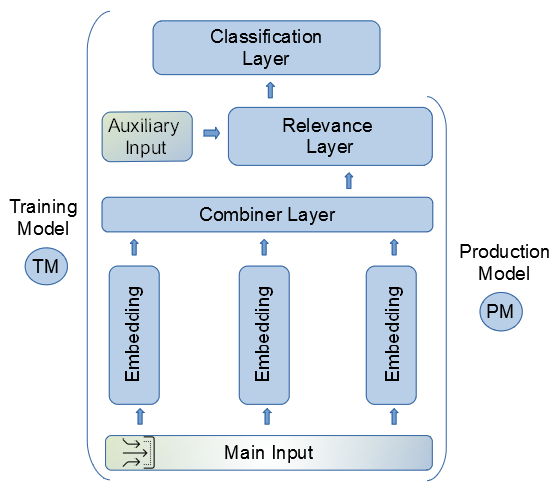
\includegraphics[width=110mm, scale = 1]{images/11_all_model.png}	
	\caption{Model Architecture}	
	\label{figure:all_model}
\end{figure}

\subsection{Data Setup \label{input_setup}}
The data obtained after the labeling step is prepared to be compatible with the neural network inputs and output labels. The inputs to the neural network are the tweet, the disease type, and disease-related labeling; these inputs are required for each member of triplet $(T_p, T_{h_1},T_{h_2})$. 
Additionally, we need the labels for the relevance between premise and the two hypotheses. These are the rankings that the labelers completed,  and become the secondary output of the network. The main output of the network is the  final binary classification of similarity which  indicates which hypothesis tweet is more similar to the premise tweet. 
 The total of data examples available was 11,425 tweets.

Each tweet is converted into a matrix, where a row is a vector in an n-dimensional embedding space that represents a word. The tweets form the 
main input to the network.
The disease group label and the disease-relatedness labels form the auxiliary input. Both of these features were binarized to change from a  categorical feature.
 In the next tweet,  we illustrate how we created the representation of the auxiliary input.

\begin{definition}
	``It is march with streets are fully covered in snow I am drinking hot milk with cocoa butter and recovering from a flu I just turned my Christmas tree lights on yes, it is still here''
\end{definition}

In the example above, the tweet mentions ``flu'', which has index 0. Suppose we have the next conditions: 0 - Flu, 1- Measles, 2- Diarrhea, and  3 - Ebola.  
We  need a bit vector with 4 entries for this. Flu is then represented 
as [1, 0, 0, 0].  This in shown on the upper left part of  Figure \ref{figure:categorical}. We have three labels for the relatedness to medical condition: 0 - not related, 1 - related, and 2- ambiguous. Here, we need a bit vector with 3 entries. Since the tweet is related with a medical condition, which is label 2, its representation 
would be [0, 1, 0]. This is shown on the upper right part of  Figure \ref{figure:categorical}. Then, for this tweet, its auxiliary representation would be the concatenation of these two bit vectors: [1, 0, 0, 0, 0, 1, 0]. This process is done
for each of the three tweets $(T_p, T_{h_1},T_{h_2})$.

\begin{figure}[H]	
	\centering
	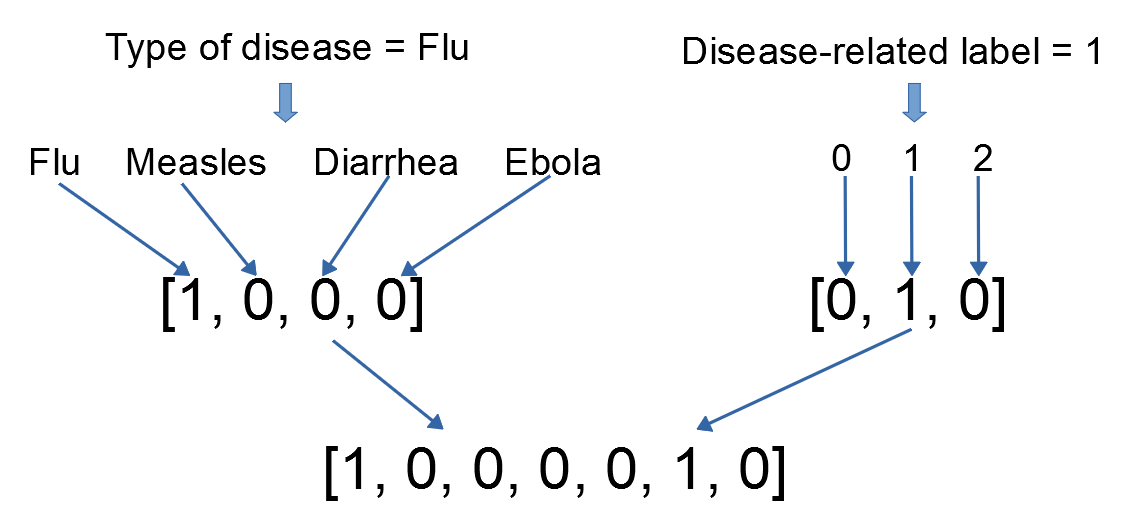
\includegraphics[width=105mm, scale = 1]{images/10_categorical.png}	
	\caption{Auxiliary Input Representation}	
	\label{figure:categorical}
\end{figure}

%\noindent Where the array with four elements is the type of disease and the array with three elements is the disease-related label. The values are binaries, it means they just can be zero or one. These two representations are combined and form the auxiliary input.

The main input of the neural network are the three tweets converted into their embedding matrices. For this purpose, our embedding layer uses GloVe embedding \cite{Pennington2014}, an unsupervised algorithm to get a vector representation for each word in the tweets. We used a pre-trained embedding that was trained with 2 billion of tweets. It is formed by a vocabulary of 1.2 million  terms with vectors of 25, 50, 100 and 200 dimensions. For our  models, we used the versions 
with 50 and 200 dimensions. Before feeding them to the neural network, the tweets were passed by a preprocessing step to remove stop words and lemmatized each word to the root lemma.


%The main input was given in two ways. The first data with all text after labeling step. Second group of data go through an additional preprocessing step to remove stop words and lemmatized each word to the root lemma.

\subsection{Combiner Layer \label{combiner_layer}}
The purpose of the combiner layer is to enable the neural network to build useful features to help it figure out how to find the similarity between tweets. 
In the early days of neural networks, features had to be engineered by hand and passed as inputs to the neural network. In contrast, modern DL approaches
rely on adding enough layer to the network so it can create the features itself. The input to the combiner network are the embedding of the tweets.
In our approach,  we implement three different combinations of algorithms that include RNN and CNN.  Each method was implemented with variation in the hyperparameters depending of each algorithm.
Finding the best hyperparameter combinations is not a trivial task. We based our experiments on the result of related researchers \cite{8622504}, and then we created our own combination, is shown in Table \ref{Hyperparameters}.

The hyperparameters variation was in epochs, learning rate, batch size, and optimizer. The hyperparameters mentioned above are not learned by the network, those ones have predefined values set before training process.

\begin{table}[htb]
	\centering
	\begin{tabular}{||M{4.5cm}|M{4cm}||}
		\hline
		\textbf{Hyperparameters} 	& \textbf{Values} 	\\ \hline
		Learning rate           	& 0.001     \\ \hline
		Epochs         				& 10, 20            \\ \hline
		Batch size           		& 32, 128 			\\ \hline		Optimizer                 	& RMSprop, Adam     \\ \hline	
	\end{tabular}
	\caption{Hyperparameter Combinations}\label{Hyperparameters}
\end{table}

\subsubsection{\ac{RNN} Combiner}
Using recurrent networks, we have two different combinations. The first implementation was a combination of two LSTM networks; they are networks with loops in them, allowing information to persist. The first LSTM network contains 128 neuron units and returns all sequences by each time step. The next LSTM network  also has 128 units, but only return the final sequence (accumulated output). The structure of this network is shown in Figure \ref{figure:lstm_only}. The same 
stack of LSTM networks is used to process the three embeddings of the tweets. $E_1$ is the embedding of $T_p$, $E_2$ is the embedding of 
$T_{h_1}$, and $E_3$ is the embedding of $T_{h_2}$.

\begin{figure}[H]	
	\centering
	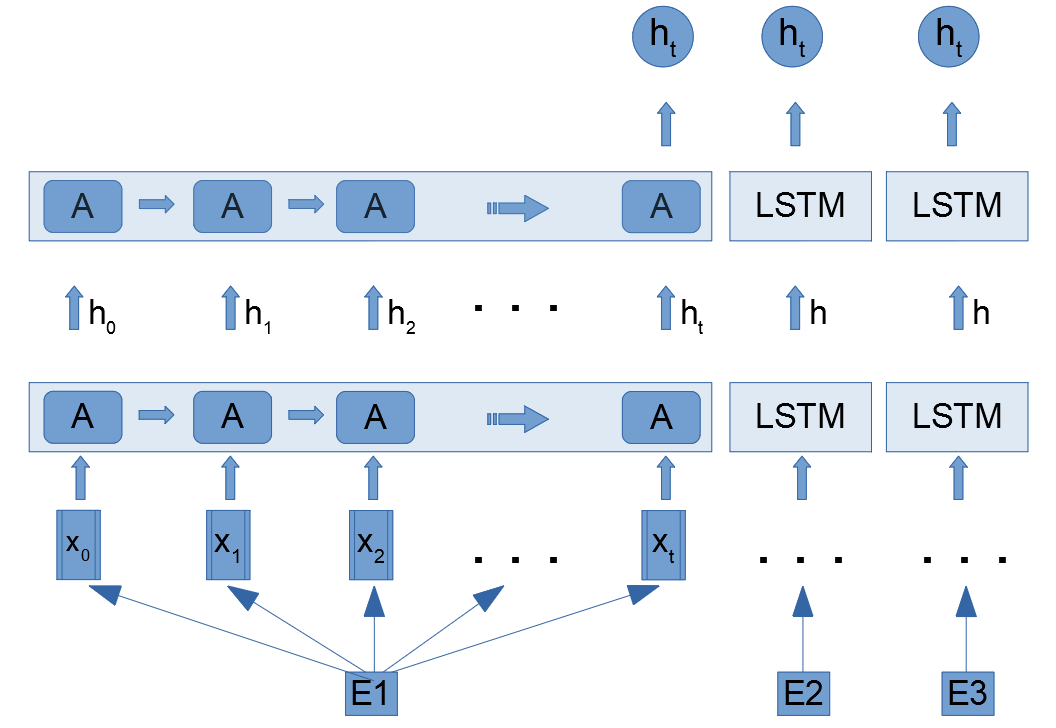
\includegraphics[width=110mm, scale = 1]{images/12_lstm_only.png}	
	\caption{Regular LSTM Network}	
	\label{figure:lstm_only}
\end{figure}

Figure \ref{figure:lstm_only} shows a double \ac{LSTM} network, where embedded tweets are the inputs and the output is a tensor with the accumulate sequence. This process is the same for each embedding vector.

Our second network implementation is a variant of \ac{LSTM} networks. In this implementation we use two sequential bidirectional LSTM networks, that consist of
 two independent \ac{LSTM} networks. The architecture is showed in Figure \ref{figure:bilstm}. In our bidirectional LSTM,  one LSTM is used to process the tweets in regular word order,  and the second one in reverse word order. Bidirectional LSTM are used to make predictions with both past and future context. 
 
 %The inputs for this layer in both networks are the embedded vectors, there are 3 vectors, one by each tweet in the triplet. The output of both two architectures are three tensors (a tensor is a data structure used how a representation of multidimensional vectors \cite{Tensor2019}), one by each tweet.

%In the bidirectional network, inputs are the same that first implementation of \ac{LSTM} network. The outputs are concatenated at each time step. concatenated output of first network is delivered to next bidirectional network. The final output only returns a tensor with the accumulated sequences. The process is repeated by each embedding. The architecture is showed in Figure \ref{figure:bilstm}


\begin{figure}[H]	
	\centering
	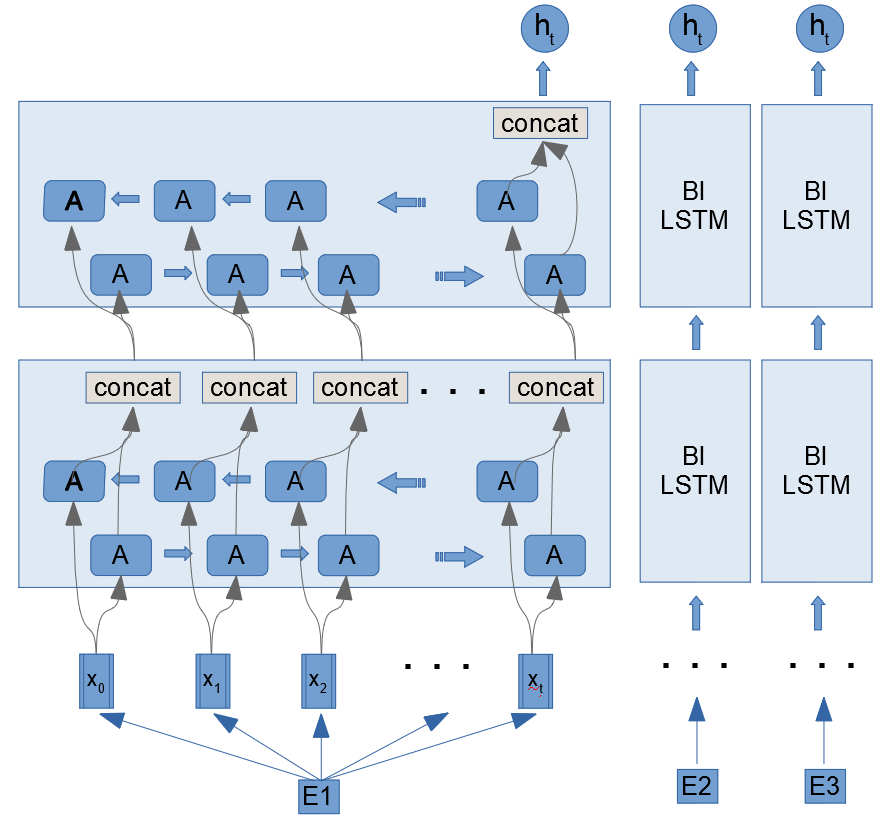
\includegraphics[width=110mm, scale = 1]{images/13_bilstm.png}	
	\caption{BiLSTM Network}	
	\label{figure:bilstm}
\end{figure}

  
\subsubsection{\ac{CNN} Combiner}

The role of a \ac{CNN} is reduce an initial sample given as a matrix into a form which is easier to process without losing features. The basic operation in this network is called ``convolution''. This operation has the objective to extract the high level features applying a filter to an input. The repeated application of the same filter results in a map of activations indicating the locations and strength of a detected feature. In this method we use the concept of inception networks. The key idea in an inception module is to deploy convolutions with multiple filters, and pooling operations in parallel within the same layer \cite{43022}. A basic inception module is showed in Figure \ref{figure:inception_module}

\begin{figure}[H]	
	\centering
	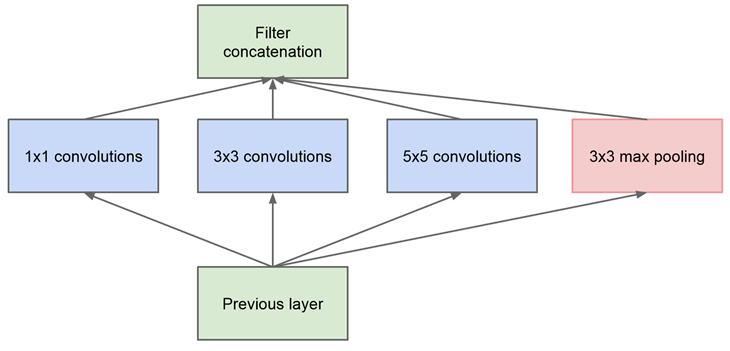
\includegraphics[width=130mm, scale = 1]{images/17_inception_module.png}	
	\caption{Inception Module as depicted in \cite{43022}.}	
	\label{figure:inception_module}
\end{figure}

Our implementation of \ac{CNN} using inception layers is showed in Figure \ref{figure:cnn_combiner}. This network follows the basic concept of an inception module using filters of 1x1, 3x3, and 5x5 convolutions. Filters with length of 5x5 passed through a zero padding layer used such that the output has the same length as the original input. Next the results of each filter are concatenated and finally we obtain a output containing the high level features of each tweet.


\begin{figure}[H]	
	\centering
	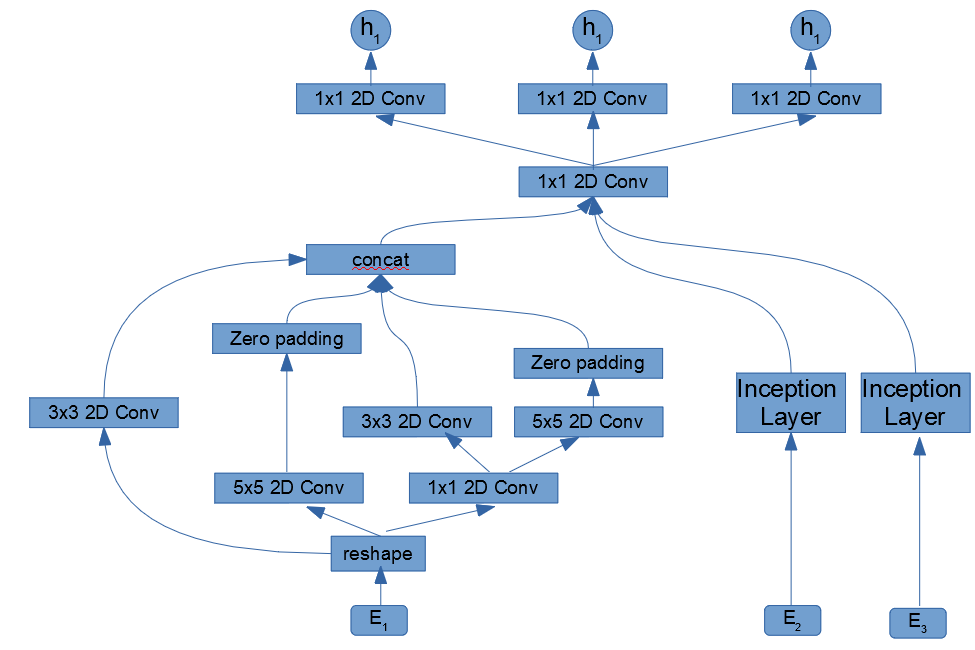
\includegraphics[width=140mm, scale = 1]{images/16_cnn_model.png}	
	\caption{Inception \ac{CNN}}	
	\label{figure:cnn_combiner}
\end{figure}

\subsection{Relevance Layer}

The input for the relevance layer are the three outputs of the combiner layer: $C_1, C_2$ and $C_3$. These tensors represent 
the output of the combiner layer for $E_1, E_2$ and $E_3$, respectively.  In the relevance layer the network tries to learn the relevance rank between tweets: 
$rank(T_p, T_{h_1})$ and $rank(T_p, T_{h_2})$.  The full structure of the relevance component is shown in Figure \ref{figure:relevance}.

To extract relationships between tweets, various methods concatenations are applied : 

\begin{itemize}
	\item $D_1 = concat(C_1*C_2, |C_1 - C_2|, C_1, C_2)$  - combines features from $T_p$ and $T_{h_1}$
	\item $D_2 = concat(C_1*C_3, |C_1 - C_3|, C_1, C_3)$  - combines features from $T_p$ and $T_{h_2}$
\end{itemize}

Where $concat()$ is a concatenation operation. 
$D_1$ is  a feature tensor build by concatenating: a) element-wise product of $C_1$ and $C_2$, b) absolute difference of $C_1$ and $C_2$, c) $C_1$ itself, 
and d) $C_2$ itself. This idea is adapted from the work in \cite{Conneau2017}. 
The same process is done with $D_2$. 
%, the method is a concatenation of premise representation, the hypothesis representation, the element-wise product and absolute element-wise difference of premise and hypothesis \cite{Conneau2017}. 
Each  tensor $D_i$ is then concatenated with the auxiliary inputs the pair of tweets used to form $D_i$ . This resulting tensor is passed through  a dense layer of 128 units with {\em \ac{ReLU}} activation and then goes into a dense layer of one unit with no activation. The result represents the similarity  $r_i$ between the premise  tweets  and the hypothesis tweet $T_{h_i}$.  The value $r_1$ gives the similarity between  $T_p$ and $T_{h_1}$, while $r_2$ gives the similarity between  $T_p$ and $T_{h_2}$.
These two values are secondary outputs to the model, and are also used in the final classification layer. 

\begin{figure}[H]	
	\centering
	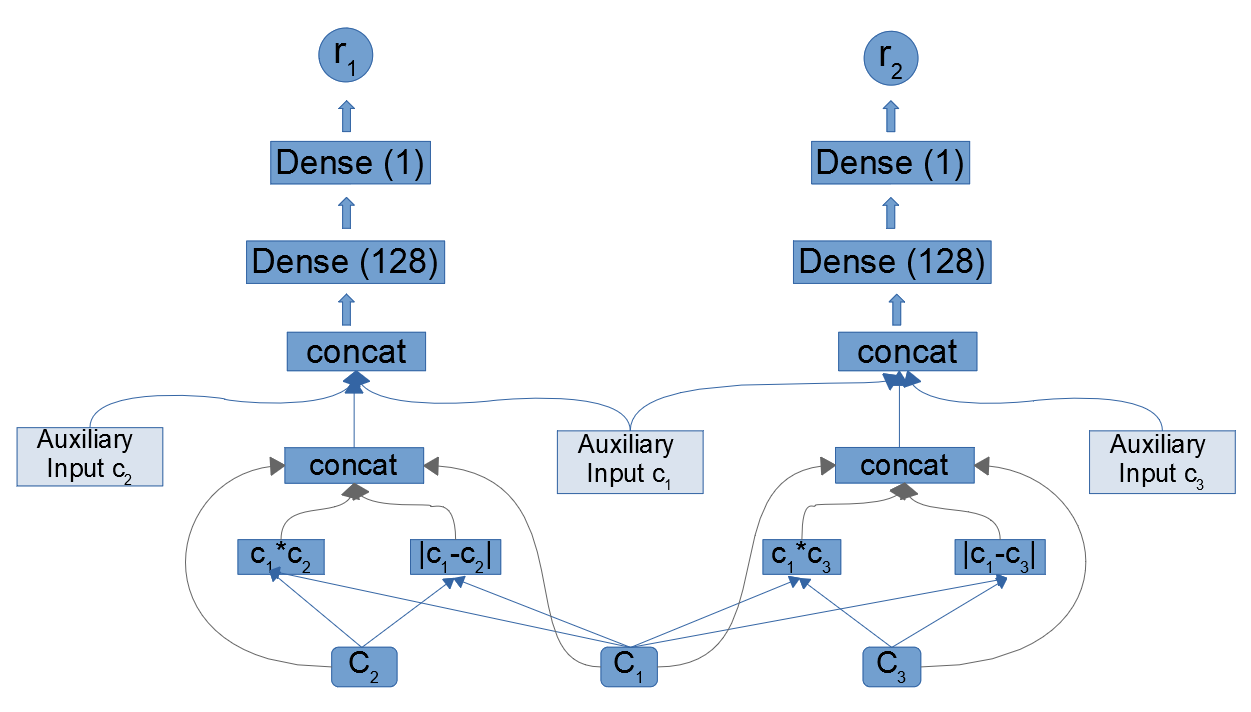
\includegraphics[width=140mm, scale = 1]{images/14_relevance.png}	
	\caption{Relevance Layer}	
	\label{figure:relevance}
\end{figure}

\subsection{Classification Layer}

The classification layer takes as input the relevance layer outputs and concatenates them. Next, this tensor is fed into  a sequence of three dense layers of 16, 8, and 1 units respectively. The dense layers with 16 and 8 units have a \ac{ReLU} activations. In the final dense layer, we use a sigmoid activation to obtain a binary output. The final output can take two values: a) 1 means the first hypothesis $T_{h_1}$ is more similar to the premise $T_p$, and b) 0 when second hypothesis 
$T_{h_2}$ is more similar to premise $T_p$. Figure \ref{figure:classification} shows the architecture of this component.

\begin{figure}[H]	
	\centering
	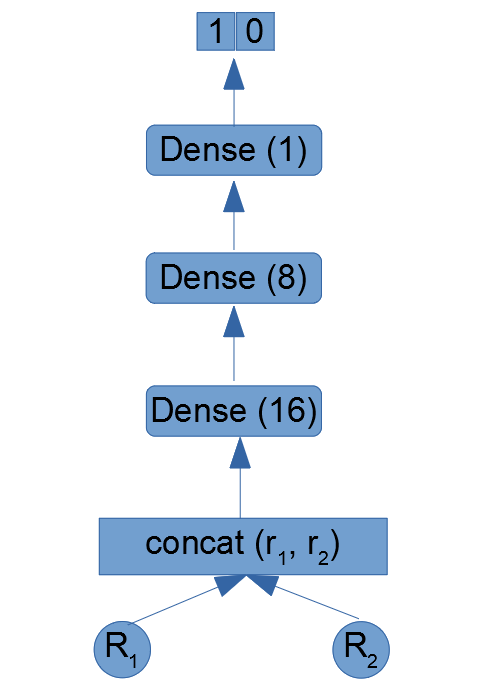
\includegraphics[width=50mm, scale = 1]{images/15_classification.png}	
	\caption{Classification Layer}	
	\label{figure:classification}
\end{figure}

\section{Metrics}
Our model has one main output and two secondary outputs: 
\begin{itemize}
	\item {\bf Main output}  - classification label to indicate which hypothesis tweet is more similar to the premise. 
	\item {\bf Secondary output \#1} - similarity between $T_p$ and  $T_{h_1}$: $rank(T_p, T_{h_1})$.
	\item {\bf Secondary output \#2} - similarity between $T_p$ and  $T_{h_2}$: $rank(T_p, T_{h_2})$.
\end{itemize} 

We use {\em accuracy} to measure the quality of  our models on the main output  since this is a classification task. Likewise, 
we use  {\em Mean Squared Error} to measure the quality of  our models on the secondary outputs since these are regression tasks. 

%\subsection{Accuracy}
%Here text
%\subsection{Mean Square Error}
%Here text
%\subsection{Loss}
%here Text

\chapter{Performance Evaluation} \label{chapter 5}
In this chapter we evaluate the quality of our \ac{DL} models by measuring their accuracy and mean squared errors on our data sets. 
\section{Hardware} 

In this research we use two different environments to run our experiments. The cluster distribution presented in Figure \ref{figure:ths_cluster} shows the components of the \ac{THS} project that was configured as described in Section \ref{ths_system}. The master-node and edge-node were set with Ubuntu 16.04 LTS \ac{OS} and data-nodes with Ubuntu 14.04 LTS \ac{OS}. These nodes are installed and run on bare metal. All operations are executed in the edge-node that connect the users with Big Data environment.

\begin{figure}[H]	
	\centering
	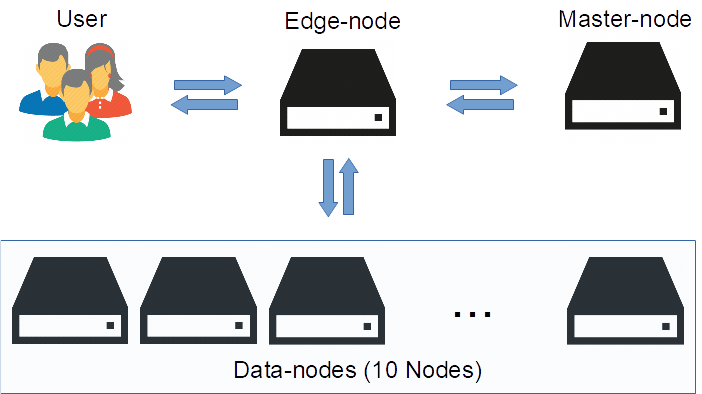
\includegraphics[width=110mm, scale = 1]{images/7_ths_cluster.png}	
	\caption{\ac{THS} Cluster}	
	\label{figure:ths_cluster}
\end{figure}

The hardware specification by each node is shown  in table \ref{node_cluster}. The total cluster storage is 2.9 TB and 80 GB of memory to processing data
(excluding master-node and edge-node). {\bf This environment was used for tweet capture, filtering, and storage}

\begin{table}[htb]
	\centering
	\begin{tabular}{||M{3.0cm}|M{4.5cm}||}
		\hline
		\textbf{Hardware} 	& \textbf{Description} \\ \hline
		Hard disk           & 297 GB            \\ \hline
		RAM          		& 8 GB              \\ \hline
		Processor           & Intel(R) Xeon(R) E3120 @ 3.16GHz  \\ \hline
		GPU                 & None              \\ \hline	
	\end{tabular}
	\caption{\ac{THS} Cluster Node}\label{node_cluster}
\end{table}

The other environment with important resources to run our experiments was Chameleon Cloud, an online large-scale platform for research, with a variety of resources in Hardware and Software. For this project we {\bf used Chameleon nodes with \ac{GPU} resources to train our \ac{DL} models}. These nodes ran in Ubuntu 16.04 LTS on bare metal. The OS image used for the project is a custom image created by \ac{THS} project. The hardware specification is described next in table \ref{node_chameleon}.

\begin{table}[htb]
	\centering
	\begin{tabular}{||M{3.0cm}|M{4.5cm}||}
		\hline
		\textbf{Hardware} 	& \textbf{Description} \\ \hline
		Hard disk           & 207 GB            \\ \hline
		RAM         		& 128 GB              \\ \hline
		Processor           & Intel(R) Xeon(R) CPU E5-2670 v3 @ 2.30 GHz x 2 \\ \hline
		GPU                 & Tesla P100 - 32GB              \\ \hline	
	\end{tabular}
	\caption{Chameleon Cloud Custom Node}\label{node_chameleon}
\end{table}

\section{Software}
The software resources used for this research are the following: 
\begin{itemize}[nolistsep]
	\item \textbf{Python:} A programming language  used in research fields, for its simplicity and power. It is compatible with tools used in this research: TensorFlow and Keras. All the code in this project is written in Python language.
	
	\item \textbf{Twitter \ac{API}:} A tool to  get data in real time from twitter for our research. 
	
	\item \textbf{\ac{HDFS}:} This software allows a distributed processing of  massive amounts of data, running in commodity hardware \cite{Hadoop2019}.
	
	\item \textbf{HIVE:} A data warehouse software for large datasets in a distributed storage. For querying, it use use \ac{SQL} syntax \cite{Hive2019}.
	
	\item \textbf{KAFKA:} It is a streaming platform to store streams of records and enables to process them asynchronously. It can be implemented in standalone mode or cluster mode. Each stream store is called a ``topic'' \cite{Kafka2019}.
	
	\item \textbf{SPARK:} Apache Spark is a fast, general purpose and unified analytic engine for large-scale data processing. It is compatible with JAVA, Scala, Python, and R. Spark support structured data processing, \ac{ML}, graph processing, and stream processing of live data \cite{Spark2019}.
	
	\item \textbf{Tensorflow:} Google's Open source \ac{ML} library for building and training complex neural network models \cite{Tensor2019}.
	
	\item \textbf{Keras:} A neural network \ac{API}, that allows easy and fast experimentation, and supports \ac{CNN} and \ac{RNN}. This tool works with Python and can be used on \ac{CPU} and \ac{GPU} \cite{Keras2019}. {\bf All \ac{ML} code in this project was implemented with Keras}.
	
	\item \textbf{\ac{CUDA}:} A programming model developed by NVIDIA; it is a parallel computing programming on \ac{GPU}, the sequential computes on thousands of cores in parallel mode, optimizing the performance of tasks \cite{Cuda2019}. TensorFlow uses CUDA to implement its neural networks. 
	
	\item \textbf{Torch: } A framework to support \ac{ML} algorithms using \ac{GPU} in a efficient way. This tool seeks to facilitate and speed up the implementation of neural network libraries and optimization packages.\\% \cite{torch2019}.\\
	
\end{itemize}


%Tools used are Open Source. Hadoop, Yarn, Spark, Kafka for \ac{THS} cluster only and Keras, TensorFlow, Tensor Board, Scikit-learn, \ac{NLTK}, SciPy and torch for both {THS} edge-node and Chameleon Cloud custom node. 
The versions of the  tools implemented in \ac{THS} project are showed in Table \ref{software_cluster} whereas the versions of software packages installed in both environments are presented in table \ref{software_packages}.

\begin{table}[htb]
	\centering
	\begin{tabular}{||M{3.0cm}|M{4.0cm}||}
		\hline
		\textbf{Software} 	& \textbf{Version} \\ \hline
		Hadoop \& Yarn   	& 2.7              \\ \hline
		Hive            	& 2.2              \\ \hline
		Spark             	& 2.1              \\ \hline
		Kafka            	& 0.10.1           \\ \hline
	\end{tabular}
	\caption{Big Data Tools in \ac{THS} System \label{software_cluster}} 
\end{table}



\begin{table}[htb]
	\centering
	\begin{tabular}{||M{3.0cm}|M{4.0cm}||}
		\hline
		\textbf{Software} 	& \textbf{Version} 	\\ 	\hline
		TensorFlow       	& 1.12.0            \\ 	\hline
		TensorBoard     	& 1.12.2            \\ 	\hline
		Keras            	& 2.2.2            	\\ 	\hline
		Scikit-learn     	& 0.19.1           	\\ 	\hline
		\ac{NLTK}           & 3.4           	\\ 	\hline
		SciPy         		& 1.1.0           	\\ 	\hline
		Torch           	& 1.0.1          	\\ 	\hline
		\ac{CUDA}			& 9.0				\\	\hline
	\end{tabular}
	\caption{Version of Software in \ac{THS} Nodes \label{software_packages}} 
\end{table}

\section{Data Collection for Training Models}

The process to collect data and prepare it for processing as  input to our models is shown in Figure \ref{figure:data_collection} and it is described in the steps following.

\begin{figure}[H]	
	\centering
	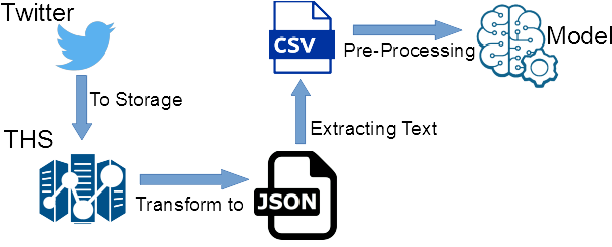
\includegraphics[width=100mm, scale = 1]{images/8_data_collection.png}	
	\caption{Data Collection Process }	
	\label{figure:data_collection}
\end{figure}

\begin{itemize}[nolistsep]
	
	\item \textbf{Step 1:} To get data from Twitter we used a Twitter Streaming \ac{API}, and we collected data and  processed it through \ac{THS} system where the tweets are stored in a Hive Database.
	
	\item \textbf{Step 2:} Running a python script we got data from  the ``raw$\_$tweet'' table of the \ac{THS} system. Here, we filtered data by specific diseases and by date, 
	using Spark tools. The tweets are saved  in a \ac{JSON} file because originally tweets have a \ac{JSON} format. This facilitates the next step of processing.
	
	\item \textbf{Step 3:} Using the  \ac{JSON}  file created in the previous step, we filtered data and only took the tweet text (sentence itself) because our project only needs to work with the text written by the user. Also, we threw away repeated tweets. This filtered data was saved in a \ac{CSV} file to next processing step.
	
	\item \textbf{Step 4:} In this step the data passes to the pre-processing step to clean and filter data before deliver data to labeling step. This process is described in Section \ref{data_preprocessing} 
	
	\item \textbf{Step 5:} The data collected is ready for labeling, and then for input to our model.
	
\end{itemize}

\section{Data Pre-processing} \label{data_preprocessing}

Data collected from social networks contains misspelling, slang, or no textual information, that makes it less structured and informal. This is the reason for cleaning the data as a previous step to build our model. This stage is composed by three demarcated steps: Pre-processing before labeling, labeling task, and final pre-processing. These steps are shown in Figure \ref{figure:data_preprocessing}. 

\begin{figure}[H]	
	\centering
	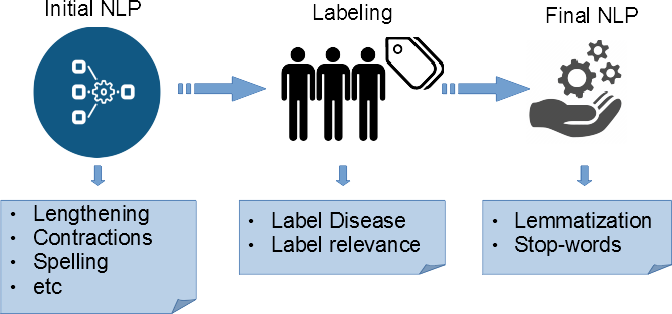
\includegraphics[width=100mm, scale = 0.8]{images/9_data_preprocessing.png}	
	\caption{Data Pre-processing}	
	\label{figure:data_preprocessing}
\end{figure}

In this section we will describe the first and last step of processing. The labeling step will be described in section \ref{data_labeling}. Before using tweets directly or labeling, it is necessary to filter and clean the data \cite{Halibas2018,Dai2017,Ahuja2017}. The operations to prepare data are described below.

\begin{itemize}[nolistsep]
	\item \textbf{Remove line breaks:} It is necessary to clean line breaks because they can be generating more than one row from the same tweet and we can lose context and meaning.
	
	\item \textbf{Remove links, hashtags and mentions:} Social media is informal and contains no textual information; this is why we cleaned no-relevant data such as links, hashtags, and mentions \cite{Dai2017}.
	
	\item \textbf{Character unescape:} We replaced source code based on hexadecimal code with the character that it represents to be understandable and compatible with human language.
	
	\item \textbf{Reduce lengthening:} Many typo errors are presented in the text like repetition of a character, many times to express emphasis or simply because there exists a typographic mistake. For example, the word ``fluuu'' represents the next word ``flu''. In cases like this one,  it needs to be fixed, and replaced with the right word.
	
	\item \textbf{Expand contractions:} To ensure a correct representation of each word, we expanded all contraction to their original form.
	
	\item \textbf{Keep text and Number:} After the previous operation, we removed all characters which are noisy to the \ac{ML} algorithm. We just conserved text and numbers.
	
	\item \textbf{Spelling corrections:} It was necessary a spelling corrector to fix typographical errors and help to avoid misunderstanding in labeling step or to process it as an unknown word in the vectorization step.\\
	
\end{itemize}

Cleaned data obtained from the previous process is ready to deliver to labeler users, from which main and auxiliary label inputs are built. This step is described in section \ref{data_labeling}.

The final \ac{NLP} steps are: 

\begin{itemize}[nolistsep]
	\item \textbf{Lemmatization:} It is a process to find a lemma for each word in a tweet. This refers to converting all inflected forms in its base form. For example, the words: ``taking'', and ``takes'' refers to base form of the word ``take''. Lemmatization considers the context and meaning to convert a word to its base form. For example in the word ``caring'' a simple stemming process will cutoff termination ``ing'' and return ``car''; in change a lemmatization process will return the word ``care''. %In other hand with lemmatization it returns “care”. 
	The better known tools are \ac{NLTK}, textBlob, spaCy, pattern, and Stanford CoreNLP. 

	\item \textbf{Remove stop-words:} The final operation of the processing step is removing the stop-words (e.g. articles, and pronouns) and just keep words with high meaning.
\end{itemize}

\section{Data Labeling} \label{data_labeling}

Since our model follows a supervised approach, it is necessary to use labeled data. In this project we have two different kinds of labeling. The first one is focused in classifying the tweets if they are related or no to a disease. The other type refers to set a measure of similarity between tweets. We now describe how they were built.
% are described following.

\subsection{Disease-Related Labeling}

The training set is composed of 11,937 tweets and it was labeled by five members of the \ac{THS} team. Labels depends on the classification in term of similar meaning and their relatedness with specific topics about health diseases. There are three possible label values for each tweet. 

\begin{itemize} [nolistsep]
	\item \textbf{0:} This label represents a tweet that is not related to a disease. 
	\item \textbf{1:} It is a tweet with meaning  related to a disease.
	\item \textbf{2:} Tweets have an ambiguous meaning, difficult to classify.
\end{itemize}

\subsection{Labeling for Level of Relevance (rank)} \label{data_relevance_labeling}

To label for relevance of similarity between tweets we built triplets ( collection of three sets). The first  dataset consisted of  11,425 triplets $(T_p, T_{h_1}, T_{h_2})$. All the tweets in these triplets were known to 
be related with a medical conditions and had one of the four target keywords: Ebola, Flu, Measles, or Diarrhea.
Labelers were asked to rank the similarity between $T_p$ and $T_{h_1}$ and between $T_p$ and $T_{h_2}$.
There were 54 labelers, which were students from UPRM. Triplets were equally divided between them.  

%The first  set that was manually labeled consists of three tweets with a common meaning, it belongs to the same disease class and their label value is 1 (``the tweet meaning is related to a disease''). The second group is form by two similar tweets and one tweet out of class, that means that last tweet is in a different class that others two; consequently, the first and second are similar, in other hand the first and the third are not similar. Finally, the last group of triplets is composed by tweets with the same class of disease, but the third tweet has a label value of 0 or 2, indicating that the tweet does not has a semantic or context relationship with the others tweets in the triplet.

%All triplets were built using the training set of 11,937 samples after labeling if it is related with a disease or no. The triplets that were labeled manually are which belongs to the first group, only tweets in the same class with label with value of 1, to know the level of relevance between similar tweets. The total of triplets labeled were 4,225; it was 1,075 triplets by each disease mentioned next ``Flu'', ``Measles'', ``Ebola'' and ``Diarrhea''. ``Zika'' was not taken in because, we do not have enough samples to build triplets. Each tweet was labeled by 3 different subjects doing a total of 12,675 samples. Triplets were equality divided between 54 collaborators.  The measure of relevance is in a range of 1 to 4, where the level of final relevance is given by the average of those three measures. While the measure is higher, it represents more similarity between the pair of tweets analyzed. 

%A metric of similarity is obtained from relevance measures. Given three tweets $t_0$, $t_1$ and $t_2$, the measure of similarity takes a value of 1 or 0; where this is 1 when $t_0$ is more similar to $t_1$ than $t_2$, and it is 0 when $t_0$ is more similar to $t_2$ than $t_1$.

Labelers were instructed to give a score between 1 and 4. The rules that were considered to manually labeling the relevance between tweets were the following:

\begin{enumerate}
	\item Score 4 - \text{When tweets discuss the same disease:}
	\begin{itemize}
		\item \textbf{Tweet 1:} \textit{There is a measles outbreak in japan.}
		\item \textbf{Tweet 2:} \textit{Japanese fear measles outbreak in progress.}
	\end{itemize}

	\item Score 3 - \text{Tweets discuss the same disease, but the events are not related:}
	\begin{itemize}
		\item \textbf{Tweet 1:} \textit{Government intensifies educational campaign against Ebola.}
		\item \textbf{Tweet 2:} \textit{Many countries launch initiatives to raise awareness about Ebola.}
	\end{itemize}

	\item Score 2 - \text{Tweets discuss the same disease at the same location:}
	\begin{itemize}
		\item \textbf{Tweet 1:} \textit{Outbreak report of Zika at Ponce.}
		\item \textbf{Tweet 2:} \textit{Government of Ponce warns about outbreak of Zika.}
	\end{itemize}
	
	\noindent Labelers were given two options for giving a score of one (1); if the tweets 

	\item Score  1 - \text{Described different symptoms of the same disease:}
	\begin{itemize}
		\item \textbf{Tweet 1:} \textit{Big headache and fever due do you the flu.}
		\item \textbf{Tweet 2:} \textit{I have been two days in bed feeling ill, due the flu}, or, 
	\end{itemize}
	
	\item Score  1 - If the tweets referred to similar action in topics related to diseases:
	\begin{itemize}
		\item \textbf{Tweet 1:} \textit{Government recommends getting the flu vaccine.}
		\item \textbf{Tweet 2:} \textit{Today I went to the pharmacy to get the flu vaccine.}
	\end{itemize}
\end{enumerate}

We  augmented the data  by adding two additional group of triplets.  In the first group, one of the 
hypothesis tweets, $T_{h_i}$ has the same disease keyword as $T_p$ but is not related to a medical condition (class 0). In this case, the 
ranking of this tweet with respect to $T_p$ is set to 0. In the second group, one of the 
hypothesis tweets, $T_{h_i}$ has a different disease keyword as that $T_p$.  In this case, the 
ranking of this tweet with respect to $T_p$ is also set to 0. In total, we grew the training data set to 11,425 tweets. 
Based on the ranking of the tweets we provide a final label $L$. This label is a classification label for relative comparison between tweets: 1 - if $rank(T_p, T_{h_1}) >= rank(T_p, T_{h_2})$, 0 - if  $rank(T_p, T_{h_1}) < rank(T_p, T_{h_2})$.


\section{Experiment Setup}
Experiments were set up in two environments with different resources: Chameleon Cloud and \ac{THS} cluster. Data acquisition and pre-processing was done
with the \ac{THS} cluster. Model training was done in Chameleon. 
%All code was developed in Python, the script permits us to collect the data from twitter using \ac{THS} system and it was pre-processing using \ac{NLP} techniques before and after labeling of data. The process of labeling has two steps, the first step is grouping the tweets by disease and label it by their semantic relation with a disease or no. The second type of labeling is related with the compute of a measure of similarity, using triplets to compare de similarity between them and get a metric of relevance that tell us what of two tweets is more like the first one.
%These two-input feed our created model. The pair of tweets referred like premise and hypothesis pass by a series of transformation to extract relations between them and finally get a measure of relevance. Along the process we use \ac{DL} approaches using \ac{LSTM} and \ac{CNN} with different variations explained in section \ref{models}, to finally build a model able to determine given two tweets how similar they are between themselves.
Figure \ref{figure:model_setup} shows an overview of the setup structure of the whole project.

\begin{figure}[H]	
	\centering
	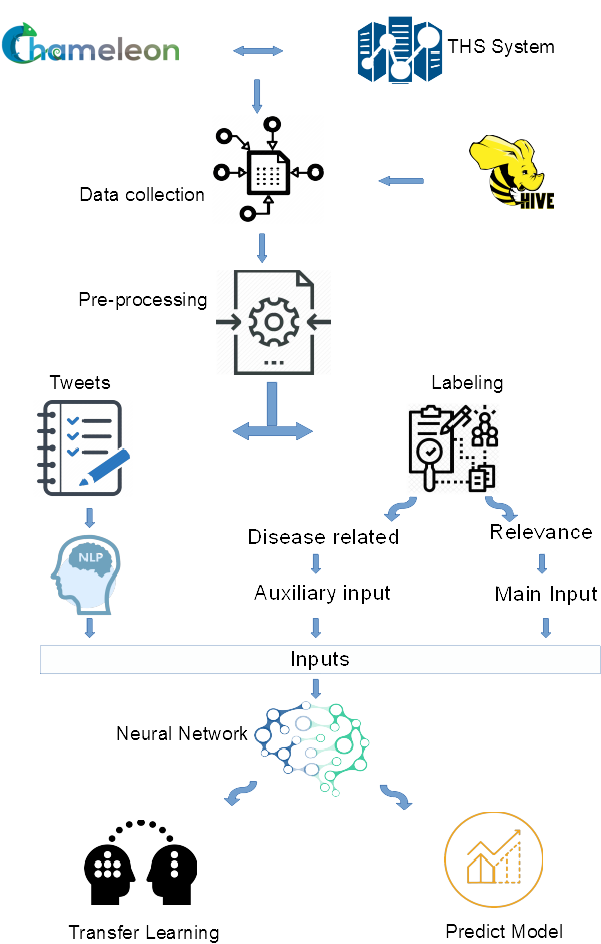
\includegraphics[height=190mm,  scale = 0.8]{images/10_architecture_setup.png}	
	\caption{Model Setup Overview}	
	\label{figure:model_setup}
\end{figure}

\subsection{Experimental Methods} \label{experimental_methods}

To train our algorithm, we mix the rows randomly to prevent order dependencies between runs and assign each example to one of these
sub-sets:

\begin{itemize}[nolistsep]
	\item \textbf{Training set}: This group comprehends 80\% of the initial data, that is 9,140 triplets. This data is used to train all combinations of algorithms presented.
	\item \textbf{Validation set}:  The remaining data is the 20\% that comprehends 2,285 samples. This data is used to validate the model by fitting the weights of parameters to find the best performance.
\end{itemize}

Usually models of \ac{ML} assume that input data has an uniform distribution between classes and do not consider the presence of imbalance data. In our case, our data is imbalanced because there are more examples classified with label 0. In our case we need to adjust our model to work with imbalanced data, because the model could be predicting in favor of the majority class. The approach taken to avoid this issue was to use a built-in functionality in Skitlearn library. This tool returns us the weights penalties for misclassifying in imbalanced clases. This approach provides a natural and straightforward method to set weight penalization.

Table \ref{class_penalties} shows the penalties by each class. A higher value is given for the minority class and a lower value to the majority class.

\begin{table}[H]
	\centering
	\begin{tabular}{||M{4.0cm}|M{3.5cm}||}
		\hline
		\textbf{Class} 	& \textbf{Penalty}		\\ \hline
		1        	& 1.181          		\\ \hline
		0 & 0.867     \\ \hline	
	\end{tabular}
	\caption{Triplets Distribution}\label{class_penalties}
\end{table}



\subsection{Results for Models using RNN at the Combiner Layer}
We divide \ac{RNN} results in two parts. First, we show those  related with \ac{LSTM} combiner and the second with bidirectional \ac{RNN} combiner. 
For RNN implementation we used an embedding vector of 50 and 200 dimensions. We used a larger embedding matrix of 200 dimensions to find out relations between tweets given to model more features. These embeddings were mentioned in section \ref{input_setup} are a pre-trained vectors of GloVe embedding.

\subsubsection{Regular LSTM}
In Table \ref{acuracy_lstm} we show the accuracy results for the \ac{LSTM}  combiner implementation. The tweet data is presented in two ways: an embedding vector taken without a preliminary preprocessing and vectors built after removing stop-words and the lemmatization process.

\begin{table}[H]
	\centering
	\begin{tabular}{||M{2.5cm}|M{2.5cm}|M{2.5cm}|M{2.5cm}|M{2.5cm}||}\hline
		\textbf{Embedding } 	& \textbf{Data Type} & \textbf{Epochs} &\textbf{Accuracy Training} & \textbf{Accuracy Validation}	\\ \hline
		50 dimensions 	& All Text   &   10 & 0.89 & 0.89		\\ \hline
		50 dimensions 	& All Text   &   20 & 0.89 & 0.88		\\ \hline
		50 dimensions 	& No Stop words and lemmatized   &   \textbf{10}	& \textbf{0.89} & \textbf{0.90}		\\ \hline
		50 dimensions 	& No Stop words and lemmatized   &   20 			& 0.90 			& 0.88		\\ \hline
		200 dimensions 	& All Text   &   10 & 0.89 & 0.89		\\ \hline
		200 dimensions 	& All Text   &   20 & 0.93 & 0.85		\\ \hline
		200 dimensions 	& No Stop words and lemmatized   &   10 & 0.90 & 0.88		\\ \hline
		200 dimensions 	& No Stop words and lemmatized   &   \textbf{20} & \textbf{0.97} & \textbf{0.86}		\\ \hline
	\end{tabular}
	\caption{Accuracy for Regular LSTM}\label{acuracy_lstm}
\end{table}

The results for accuracy metric are similar. The accuracy in the training step is in the range between 89\% and 97\%. The accuracy in the validation step is in the range between 85\% and 90\%. The next configuration has the better  accuracy metrics:

\begin{itemize}[nolistsep]
	\item 50 dimensions, 10 epochs, after lemmatization step, and rmsprop optimizer with 89\% and 90\% of accuracy in training and validation, respectively.
	\item 200 dimensions, 20 epochs, after lemmatization process, rmsprop optimizer with 97\% and 86\% of accuracy for training and validation, respectively.
\end{itemize}
The case of 50 dimensions, 10 epochs, rmsprop optimizer, and after lemmatization step provided best accuracy on validation and it is the selected model. 

In table \ref{loss_lstm} we show measures for the loss functions. We used Mean Squared Error (MSE) loss function in  the ranking outputs and cross-entropy loss function for final classification of triplets. MSE measures the average of the squares of the errors in our model. For the best model the MSE metrics were 0.37 and 0.34 of training and validation, respectively.

\begin{table}[H]
	\centering
	\begin{tabular}{||M{1.0cm}|M{2.5cm}|M{1.5cm}|M{2.0cm}|M{2.0cm} |M{2.0cm} |M{2.0cm}||}\hline
		\textbf{Dims } 	& \textbf{Data Type} & \textbf{Epochs} & \textbf{MSE Training} & \textbf{Cross-Entropy Training} & \textbf{MSE Validation} & \textbf{Cross-Entropy Training} 	\\ \hline
		50 	& All Text   &   10 & 0.37 & 0.23 & 0.34 & 0.23		\\ \hline
		50 	& All Text   &   20 & 0.36 & 0.21 & 0.36 & 0.24		\\ \hline
		50 	& No Stop words and lemmatized   &   \textbf{10}	& \textbf{0.37} & \textbf{0.23}	& \textbf{0.34} & \textbf{0.22}	\\ \hline
		50	& No Stop words and lemmatized   &   20 			& 0.36 			& 0.21	& 0.35 & 0.24	\\ \hline
		200 & All Text   &   10 & 0.38 & 0.22	& 0.36 & 0.24	\\ \hline
		200 & All Text   &   20 & 0.38 & 0.15	& 0.38 & 0.35	\\ \hline
		200 & No Stop words and lemmatized   &   10 & 0.38 & 0.20	& 0.36 & 0.25	\\ \hline
		200 & No Stop words and lemmatized   &   \textbf{20} & \textbf{0.41} & \textbf{0.07} & \textbf{0.41} & \textbf{0.43}		\\ \hline
	\end{tabular}
	\caption{Loss Metrics for Regular LSTM}\label{loss_lstm}
\end{table}

\subsubsection{Bidirectional \ac{RNN}}
In table \ref{accuracy_birnn} is presented the accuracy outputs for Bidirectional {RNN} implementation. As we explained in Section \ref{combiner_layer}, our Bidirectional network is composed by two bidirectional {LSTM} networks.

\begin{table}[H]
	\centering
	\begin{tabular}{||M{2.5cm}|M{2.5cm}|M{2.5cm}|M{2.5cm}|M{2.5cm}||}\hline
		\textbf{Embedding } 	& \textbf{Data Type} & \textbf{Epochs} &\textbf{Accuracy Training} & \textbf{Accuracy Validation}	\\ \hline
		50 dimensions 	& All Text   &   10 & 0.96 & 0.86		\\ \hline
		50 dimensions 	& All Text   &   20 & 0.99 & 0.86		\\ \hline
		50 dimensions 	& No Stop words and lemmatized   &  10	& 0.97 & 0.86 \\ \hline
		50 dimensions 	& No Stop words and lemmatized   &   20 & 0.99 			& 0.85		\\ \hline
		200 dimensions 	& All Text   &   10 & 0.99 & 0.86		\\ \hline
		200 dimensions 	& All Text   &   20 & 0.99 & 0.86		\\ \hline
		200 dimensions 	& No Stop words and lemmatized   &   10 & 0.99 & 0.86		\\ \hline
		200 dimensions 	& No Stop words and lemmatized   &   \textbf{20} & \textbf{0.99} & \textbf{0.87}		\\ \hline
	\end{tabular}
	\caption{Accuracy Bidirectional Network}\label{accuracy_birnn}
\end{table}

The results for accuracy metric are similar. The accuracy in training step is in the range between 96\% and 99\%. The accuracy in validation step is in the range between 85\% and 87\%. The better accuracy metrics have the next configuration:

\begin{itemize}[nolistsep]
	\item 200 dimensions, 20 epochs and after lemmatization step, rmsprop optimizer with an accuracy of 99\% and 87\% in training and validation, respectively.
\end{itemize}
Notice that the models with bidirectional LSTM in the combiner tend to overfit the input. 

In table \ref{loss_birnn} we show measures for loss functions. We used Mean Squared Error (MSE) loss function in the relevance rank outputs and cross-entropy loss function for final classification of triplets. 

\begin{table}[H]
	\centering
	\begin{tabular}{||M{1.0cm}|M{2.5cm}|M{1.5cm}|M{2.0cm}|M{2.0cm} |M{2.0cm} |M{2.0cm}||}\hline
		\textbf{Dims } 	& \textbf{Data Type} & \textbf{Epochs} & \textbf{MSE Training} & \textbf{Cross-Entropy Training} & \textbf{MSE Validation} & \textbf{Cross-Entropy Training} 	\\ \hline
		50 	& All Text   &   10 & 0.39 & 0.10 & 0.40 & 0.41		\\ \hline
		50 	& All Text   &   20 & 0.35 & 0.02 & 0.41 & 0.77		\\ \hline
		50 	& No Stop words and lemmatized  &  \textbf{10}	& 0.39 & 0.08 & 0.40 & 0.44	\\ \hline
		50	& No Stop words and lemmatized   &   20 			& 0.35 			& 0.02	& 0.39 & 0.80	\\ \hline
		200 & All Text   &   10 & 0.38 & 0.03	& 0.43 & 0.61	\\ \hline
		200 & All Text   &   20 & 0.31 & 0.01	& 0.36 & 0.76	\\ \hline
		200 & No Stop words and lemmatized   &   10 & 0.36 & 0.02	& 0.39 & 0.66	\\ \hline
		200 & No Stop words and lemmatized   &   \textbf{20} & \textbf{0.28} & \textbf{0.01} & \textbf{0.35} & \textbf{0.78}		\\ \hline
	\end{tabular}
	\caption{Loss Bidirectional Network}\label{loss_birnn}
\end{table}

\subsection{Results for Models using CNN at the Combiner Layer}

For the \ac{CNN} implementation we also used an embedding vector of 50 and 200 dimensions. We  used the Inception network approach, a complex and heavily engineered \ac{CNN} network. It used a lot of tricks to push performance, in terms of speed and accuracy. The network essentially would get wider rather than deeper, in order  to tackle the issue of overfitting. The network structure is described in section \ref{combiner_layer}.

In table \ref{accuracy_cnn} is presented the accuracy outputs for Inception CNN implementation.

\begin{table}[H]
	\centering
	\begin{tabular}{||M{2.5cm}|M{2.5cm}|M{2.5cm}|M{2.5cm}|M{2.5cm}||}\hline
		\textbf{Embedding } 	& \textbf{Data Type} & \textbf{Epochs} &\textbf{Accuracy Training} & \textbf{Accuracy Validation}	\\ \hline
		50 dimensions 	& All Text   &   10 & 0.97 & 0.85		\\ \hline
		50 dimensions 	& All Text   &   \textbf{20} & \textbf{0.99} & \textbf{0.86}		\\ \hline
		50 dimensions 	& No Stop words and lemmatized   &  10	& 0.95 & 0.85 \\ \hline
		50 dimensions 	& No Stop words and lemmatized   &   20 & 0.99 			& 0.84		\\ \hline
		200 dimensions 	& All Text   &   10 & 0.98 & 0.84		\\ \hline
		200 dimensions 	& All Text   &   \textbf{20} & \textbf{0.99} & \textbf{0.87}		\\ \hline
		200 dimensions 	& No Stop words and lemmatized   &   10 & 0.97 & 0.86		\\ \hline
		200 dimensions 	& No Stop words and lemmatized   &   20 & 0.99 & 0.86		\\ \hline
	\end{tabular}
	\caption{Accuracy CNN Model}\label{accuracy_cnn}
\end{table}

In general the metrics for accuracy are very close. The higher value was when the tweets only passed the first pre-processing (without remove stop-words or lemmatization process). The accuracy in training step is in the range between 95\% and 99\%. The accuracy in validation step is in the range between 84\% and 87\%. The better accuracy metrics have the next configuration:

\begin{itemize}[nolistsep]
	\item 50 dimensions, 20 epochs and before lemmatization step, rmsprop optimizer with an accuracy of 99\% and 86\% in training and validation, respectively.
	\item 200 dimensions, 20 epochs and before lemmatization step, adam optimizer with an accuracy of 99\% and 87\% in training and validation, respectively.
\end{itemize}

In table \ref{loss_cc} we show measures for loss functions. We used Mean Squared Error (MSE) loss function in relevance parameters and cross-entropy loss function for final classification of triplets. 

\begin{table}[H]
	\centering
	\begin{tabular}{||M{1.0cm}|M{2.5cm}|M{1.5cm}|M{2.0cm}|M{2.0cm} |M{2.0cm} |M{2.0cm}||}\hline
		\textbf{Dims } 	& \textbf{Data Type} & \textbf{Epochs} & \textbf{MSE Training} & \textbf{Cross-Entropy Training} & \textbf{MSE Validation} & \textbf{Cross-Entropy Training} 	\\ \hline
		50 	& All Text   &   10 & 0.42 & 0.08 & 0.47 & 0.43		\\ \hline
		50 	& All Text   &   \textbf{20} & \textbf{0.24} & \textbf{0.02} & \textbf{0.34} & \textbf{0.75}		\\ \hline
		50 	& No Stop words and lemmatized  &  10	& 1.48 & 0.12 & 1.41 & 0.37	\\ \hline
		50	& No Stop words and lemmatized   &   20 			& 1.34 			& 0.03	& 1.29 & 0.66	\\ \hline
		200 & All Text   &   10 & 1.56 & 0.06	& 1.54 & 0.53	\\ \hline
		200 & All Text   &   \textbf{20} & \textbf{1.33} & \textbf{0.02}	& \textbf{1.35} & \textbf{0.66}	\\ \hline
		200 & No Stop words and lemmatized   &   10 & 1.51 & 0.08	& 1.48 & 0.45	\\ \hline
		200 & No Stop words and lemmatized   &   \textbf{20} & 1.31 & 0.03 & 1.29 & 0.59		\\ \hline
	\end{tabular}
	\caption{Loss CNN Model}\label{loss_cc}
\end{table}


%\subsection{Inference Model}
%
%In our project we development two model simultaneasly, a trainig model and a production model, while we were training our model, also we were training a production model, with the goal to use for prediction a metric of relevance. Given a premise tweet the model can be look in stream of tweets and order them by similarity.
%As and example we show an experiment with following premise tweet:
%
%\begin{definition}
%	``Here tweet''
%\end{definition}
%
%The result for five closer tweets to premise are the showed following. They ordered in a descendant way
%
% \begin{itemize}[nolistsep]
% 	\item tweet 1
% 	\item t2
% 	\item t3
% 	\item t4
% 	\item t5
% \end{itemize}

\subsection{Discussion of Results}

In the results for models  the \ac{RNN} combiner we concluded that the best performing in accuracy  is a model regular LSTM combiner with an embedding using 50 dimensions, with text processed after lemmatization, 10 epochs, batch size of 32 and rmsprop optimizer. The results show a training accuracy of 89\% in training and 90\% in validation step. The loss metrics were 0.37 and 0.34 for {MSE} in training and validation. The cross-entropy loss function in this configuration had 0.23 for training step and 0.22 in validation.

In the case of {CNN} approach the best model are close among them and not distant from the \ac{RNN} results, both having a high accuracy for training. The configuration of hyperparameters for the best model had an embedding with  200 dimensions, text before lemmatization and without remove stop words, batch size of 32 and adam optimizer. The measured of accuracy in training was 99\% and 87\% for validation. {MSE} in training had a value of 1.33 and 1.3. On the other hand Cross-entropy loss had 0.02 in training and 0.66 in validation. 

%Notice that the best result of the bidirectional \ac{RNN} approach have the same measures for accuracy as the best models with \ac{CNN}. 

%The Intern hyperparamters (e.g. number of units, size of inception kernel) for {RNN} networks and CNN were described in section \ref{combiner_layer}.
%the running time of models depend of number of epoch and batch size. In general terms the order of execution time of the three models presented is the next, inception {CNN} like the fastest, after classic {LSTM} in second place and finally with worst time execution is Bidirectional {LSTM} networks.

Comparing \ac{RNN} and \ac{CNN} results, we can see that {RNN} with two {LSTM} network joined sequentially have more consistency in training and validation accuracy, because the metric for accuracy are 89\% and 90\% in training and validation, respectively. 
Notice that the best result of the bidirectional \ac{RNN} approach have the same measures for accuracy as the best models with \ac{CNN}.  The tradeoff is 
that \ac{CNN} required less time to train. In general terms the order of training time of the three approaches presented is the next, inception {CNN} is the fastest, next is the regular \ac{LSTM} in second place, and finally, with worst time execution, is Bidirectional {LSTM} networks.


%Nonetheless, the {CNN} model is better in training accuracy and execution time.

\chapter{Conclusion and Future Work} \label{chapter 6}
In this project we used social networks as an application to get valuable information about health topics. In our case we used Twitter and its  vast amounts of data on different topics. We illustrated how to use tweet data about medical conditions to build models that are able to compute the similarity in tweets. We use the {THS} system to store data and then use it as our input data.

We used neural network employing supervised learning approach in text similarity. We showed that trained models with labeled data in sentence similarity have good performance to be widely adopted for tweet similarity and in others \ac{NLP} tasks. We build models with deep \ac{CNN} and \ac{RNN}  obtaining good results with approximately 90\% on validation step.

We trained a model to compute the similarity rank between two tweets, by first training a bigger model $M'$ capable of classifying relative similarity in triplets of tweets. We trained a bigger model that classifies which of two tweets is more similar to a premise tweet, but we use a sub-task (sub-model) $M$ to predict a relevance metric between  two tweets. This model $M$ can then be used to produce similarity scores and order a list of tweets by similarity respect to a premise tweet.

In order to validate our model we presented a performance study on the DL similarity models with a data sets consisting of 11,425 examples, and we used that data set to train our models. Our results showed that we can achieve 90\% accuracy on the task of classifying which of two tweets is more similar to a premise tweet. The sub-model $M$ trained have a 0.34 units of Mean Squared Error on a decreasing loss.

Future work can be focused in training models with more data to avoid problems of overfitting, which enable us compare with the previous models. 
Build a dataset with equally distributed labels for the relevance metric.
Also, you can explore new architecture models in {RNN} and {CNN} approaches to using in combiner layer and determine if they improve in accuracy performance. 
Furthermore use metrics of distance like Frobenius distance or cosine similarity in the relevance layer to have to different ways to measure the similarity.


%\chapter*{References} 
%\addcontentsline{toc}{chapter}{Bibliography}
\bibliographystyle{unsrt}
\bibliography{references} 
%\printbibliography[heading=none, ]

\begin{appendices}
\chapter{GitHub Repositories}
The GitHub repositories of the big data and machine learning deamon are avaliable upon request at danny.villanueva1@upr.edu. The following sections contain the links.

\section{Big Data Platform}
https://github.com/THSUPRM/bigdata/tree/master/python

\subsection{Machine Learning Platform}
https://github.com/THSUPRM/bigdata/tree/master/DetectDiseaseTHS/ths
\end{appendices}

\end{document}
